%\input{../header}
%%% DOCUMENT TYPE %%%%%%%%%%%%%%%%%%%%%%%%%%%%%%%%%%%%%%%%%%%%%%%%%%%%%%%%%%%%%%

\documentclass[11pt, a4paper]{article}

%%% PACKAGES %%%%%%%%%%%%%%%%%%%%%%%%%%%%%%%%%%%%%%%%%%%%%%%%%%%%%%%%%%%%%%%%%%%

% Encoding

\usepackage[utf8]{inputenc}
\usepackage[T1]{fontenc}
\usepackage{lmodern}

% Geometry

\usepackage{geometry} % edit margins of paper
\usepackage{setspace} % edit line spacing
\usepackage{fancyhdr} % header, footer
\usepackage{titlesec} % edit format of titles

% Images
\usepackage[pdftex]{graphicx} % image locations

% Visual

\usepackage[dvipsnames]{xcolor} % colors
\usepackage{pgf,tikz} % graphics
\usetikzlibrary{quotes}
\usetikzlibrary{cd}
\usetikzlibrary{babel}

\usepackage[framemethod=tikz]{mdframed} % frames, better theorems

% Math

\usepackage{amsmath} % math tools
\usepackage{amssymb} % math symbols
\usepackage{amsthm} % thereoms
\usepackage{mathtools} % math tools
\usepackage{xfrac} %More Fractions

% Referencing

\usepackage{nameref}
\usepackage{hyperref}
\usepackage{cleveref}

% Useful

\usepackage[shortlabels]{enumitem} % enumerations

% Other

\usepackage{lastpage} % get number of last page
\usepackage{physics}
%\usepackage{bbm}
\usepackage[makeroom]{cancel} %crossing stuff out
\usepackage{stmaryrd}
\usepackage{tabu}

%%% MARGINS %%%%%%%%%%%%%%%%%%%%%%%%%%%%%%%%%%%%%%%%%%%%%%%%%%%%%%%%%%%%%%%%%%%%

\geometry{a4paper, left=25mm, right=25mm, top=10mm, bottom=20mm, includehead}

%%% COLORS %%%%%%%%%%%%%%%%%%%%%%%%%%%%%%%%%%%%%%%%%%%%%%%%%%%%%%%%%%%%%%%%%%%%%

%%% TITLES %%%%%%%%%%%%%%%%%%%%%%%%%%%%%%%%%%%%%%%%%%%%%%%%%%%%%%%%%%%%%%%%%%%%%

\colorlet{color-section}                {BrickRed}
\colorlet{color-subsection}             {BrickRed}

%%% MATH BOXES %%%%%%%%%%%%%%%%%%%%%%%%%%%%%%%%%%%%%%%%%%%%%%%%%%%%%%%%%%%%%%%%%

\colorlet{color-definition}             {SpringGreen!20}
\colorlet{color-theorem}                {Apricot!13}
\colorlet{color-proposition}            {Apricot!13}
\colorlet{color-corollary}              {Apricot!13}
\colorlet{color-lemma}                  {Apricot!13}
\colorlet{color-attention}              {OrangeRed!13}
\colorlet{color-remark}                 {Gray!5}
\colorlet{color-example}                {Lavender!7}
\colorlet{color-notation}               {Gray!5}
\colorlet{color-convention}             {Gray!5}
\colorlet{color-claim}                  {SkyBlue!7}
% \colorlet{color-proof}                  {FILL COLOR HERE}


%%% CAPTIONS %%%%%%%%%%%%%%%%%%%%%%%%%%%%%%%%%%%%%%%%%%%%%%%%%%%%%%%%%%%%%%%%%%%

%%% CAPTION DEFINITION %%%%%%%%%%%%%%%%%%%%%%%%%%%%%%%%%%%%%%%%%%%%%%%%%%%%%%%%%

\newcommand*{\definitionname}{Definition}
\newcommand*{\theoremname}{Theorem}
\newcommand*{\propositionname}{Proposition}
\newcommand*{\corollaryname}{Corollary}
\newcommand*{\lemmaname}{Lemma}
\newcommand*{\remarkname}{Remark}
\newcommand*{\examplename}{Example}
\newcommand*{\attentionname}{Attention}
\newcommand*{\notationname}{Notation}
\newcommand*{\conventionname}{CConvention}
\newcommand*{\claimname}{Claim}


%%% SHORTCUTS %%%%%%%%%%%%%%%%%%%%%%%%%%%%%%%%%%%%%%%%%%%%%%%%%%%%%%%%%%%%%%%%%%

%%% SINGLE SYMBOLS %%%%%%%%%%%%%%%%%%%%%%%%%%%%%%%%%%%%%%%%%%%%%%%%%%%%%%%%%%%%

% Logic

% \forall exists
% \exists exists
% \lnot exists
% \lor exists
% \land exists
\newcommand*{\limp}{\rightarrow}
\newcommand*{\limps}{\; \limp \;} % \limp with some space around
\newcommand*{\leqv}{\leftrightarrow}
\newcommand*{\leqvs}{\; \leqvs \;} % \leqv with some space around
\newcommand*{\lTri}{\vartriangleleft}
\newcommand*{\on}[1]{\operatorname{#1}}
\newcommand*{\fg}{f\mathcal{G}}
% Meta Logic

% \implies exists
% \iff exists

% Colon Stuff

\newcommand*{\cl}{\colon}
\newcommand*{\cleq}{\coloneqq}
\newcommand*{\eqcl}{\eqqcolon}

% Sets

\newcommand*{\N}{\mathbb{N}} % natural numbers
\newcommand*{\Z}{\mathbb{Z}} % integers
\newcommand*{\Q}{\mathbb{Q}} % rational numbers
\newcommand*{\R}{\mathbb{R}} % real numbers
\newcommand*{\C}{\mathbb{C}} % complex numbers
\newcommand*{\F}{\mathbb{F}} % finite field

%%% MATH OPERATORS %%%%%%%%%%%%%%%%%%%%%%%%%%%%%%%%%%%%%%%%%%%%%%%%%%%%%%%%%%%%%

% General

\DeclareMathOperator{\id}{id}
\DeclareMathOperator{\sgn}{sgn}
%Analysis
\DeclareMathOperator{\vol}{vol}
\DeclareMathOperator{\supp}{supp}
\let\grad\relax
\DeclareMathOperator{\grad}{grad}
\DeclareMathOperator{\rot}{rot}
\let\div\relax
\DeclareMathOperator{\div}{div}
%LinAlg
\let\ker\relax
\DeclareMathOperator{\ker}{Ker}
\DeclareMathOperator{\eig}{Eig}
\DeclareMathOperator{\im}{Im}
\let\hom\relax
\DeclareMathOperator{\hom}{Hom}
\DeclareMathOperator{\End}{End}
\DeclareMathOperator{\mat}{Mat}
%Algebra
\let\gcd\relax
\DeclareMathOperator{\gcd}{ggT}
\let\ev\relax
\DeclareMathOperator{\ev}{ev}
\DeclareMathOperator{\charak}{char}
\DeclareMathOperator{\quot}{Quot}
\DeclareMathOperator{\sym}{Sym}
\DeclareMathOperator{\bij}{Bij}
\DeclareMathOperator{\GL}{GL}
\DeclareMathOperator{\SL}{SL}
\DeclareMathOperator{\gal}{Gal}
\DeclareMathOperator{\aut}{Aut}
\DeclareMathOperator{\out}{Out}
\DeclareMathOperator{\SO}{SO}
\DeclareMathOperator{\irr}{irr}
%%% TEMPLATES %%%%%%%%%%%%%%%%%%%%%%%%%%%%%%%%%%%%%%%%%%%%%%%%%%%%%%%%%%%%%%%%%%

% General

% write a set definition like: { #1 | #2 }
\newcommand*{\sdef}[2]{
  \{#1 \mid #2\}
}

% write a nice map definition
\newcommand*{\mdef}[5]{
  \begin{align*}
    #1 \cl #2 &\to     #3 \\
           #4 &\mapsto #5
  \end{align*}
}

\newcommand*{\nstack}[2]{
	\begin{array}{c}
		#1\\
		#2\\
	\end{array}
}


%%% FORMATTING %%%%%%%%%%%%%%%%%%%%%%%%%%%%%%%%%%%%%%%%%%%%%%%%%%%%%%%%%%%%%%%%%

%%% HEADER, FOOTER %%%%%%%%%%%%%%%%%%%%%%%%%%%%%%%%%%%%%%%%%%%%%%%%%%%%%%%%%%%%%

\pagestyle{fancy}
\renewcommand{\headrule}{}
%\renewcommand{\chaptermark}[1]{\markboth{#1}{}}
\fancyhf{} % clear everything
%\fancyhead[L]{\rightmark}
%\chead{\bfseries Zusammenfassung Algebra I/II}
%\rhead{Seite \thepage /\pageref*{LastPage}}
%\lfoot{}
\fancyfoot[C]{\thepage}
%\fancyfoot[R]{\thepage}

%%% TITLE FORMAT %%%%%%%%%%%%%%%%%%%%%%%%%%%%%%%%%%%%%%%%%%%%%%%%%%%%%%%%%%%%%%%

\setcounter{secnumdepth}{2}

%\titleformat{\chapter}[hang]
%{\normalfont\huge\bfseries}{\chaptertitlename\ \thechapter:}{20pt}{\Huge}
\titleformat{\section}
{\normalfont\LARGE\bfseries}{\thesection}{1em}{}
\titleformat{\subsection}
{\normalfont\large\bfseries}{\thesubsection}{1em}{}
\titleformat{\subsubsection}
{\normalfont\normalsize\bfseries}{\thesubsubsection}{1em}{}
\titleformat{\paragraph}[runin]
{\normalfont\normalsize\bfseries}{\theparagraph}{1em}{}
\titleformat{\subparagraph}[runin]
{\normalfont\normalsize\bfseries}{\thesubparagraph}{1em}{}

%%% SPACING %%%%%%%%%%%%%%%%%%%%%%%%%%%%%%%%%%%%%%%%%%%%%%%%%%%%%%%%%%%%%%

% Titles

%\titlespacing*{\chapter}{0pt}{0pt}{15pt}
\titlespacing*{\section}{0pt}{3.5ex plus 1ex minus .2ex}{2.3ex plus .2ex}
\titlespacing*{\subsection}{0pt}{3.25ex plus 1ex minus .2ex}{1.5ex plus .2ex}
\titlespacing*{\subsubsection}{0pt}{3.25ex plus 1ex minus .2ex}{1.5ex plus .2ex}
\titlespacing*{\paragraph}{0pt}{1.25ex plus 1ex minus .2ex}{1em}
\titlespacing*{\subparagraph}{\parindent}{3.25ex plus 1ex minus .2ex}{1em}

% Text, Paragraphs

\setstretch{1.05} % scaling of space between lines
\setlength{\parindent}{0pt} % indentation of paragraphs
\setlength{\parskip}{4.0pt plus 1.0pt minus 1.0pt} % space between paragraphs
%\setlength{\parskip}{0pt}

%%% SYMBOLS USED BY NUMBERINGS, ENVIRONMENTS, ... %%%%%%%%%%%%%%%%%%%%%%%%%%%%%%

% \renewcommand*\qedsymbol{$\blacksquare$} % alternative QED symbol
%\renewcommand{\thefootnote}{\arabic{footnote}} % normal footnotes on page
%\renewcommand{\thempfootnote}{\fnsymbol{mpfootnote}} % footnotes on minipages, e.g. in mdframed environments

%%% LISTS, ENUMERATIONS %%%%%%%%%%%%%%%%%%%%%%%%%%%%%%%%%%%%%%%%%%%%%%%%%%%%%%%%

% 'itemize'

\setlist[itemize]{noitemsep, topsep=0pt}

% 'enumerate'

\setlist[enumerate]{noitemsep, topsep=0pt}
% no special settings at the moment

% 'description'

% no special settings at the moment

% 'axioms'

%\newlist{axioms}{enumerate}{2}
%\setlist[axioms]{itemsep=0pt,label*=\arabic*.}

%%% GENERAL SYMBOLS %%%%%%%%%%%%%%%%%%%%%%%%%%%%%%%%%%%%%%%%%%%%%%%%%%%%%%%%%%%%
\newcommand\danger{\raisebox{\depth}{{\fontencoding{U}\fontfamily{futs}\selectfont\char 66\relax}}}
\newcommand\contra{\scalebox{1.5}{$\lightning$}}

%%% MDFRAMED PATCH %%%%%%%%%%%%%%%%%%%%%%%%%%%%%%%%%%%%%%%%%%%%%%%%%%%%%%%%%%%%%

\usepackage{xpatch}

\makeatletter
\xpatchcmd{\endmdframed}
  {\aftergroup\endmdf@trivlist\color@endgroup}
  {\endmdf@trivlist\color@endgroup\@doendpe}
  {}{}
\makeatother

%%% MDFRAMED STYLES %%%%%%%%%%%%%%%%%%%%%%%%%%%%%%%%%%%%%%%%%%%%%%%%%%%%%%%%%%%%

% thick frame and bar for title

%\mdfdefinestyle{style-box}{
%  skipabove=1.5ex plus .5ex minus .2ex,
%  skipbelow=1ex plus .2ex minus .2ex,
%  linewidth=2pt,
%  linecolor=Gray!20,
%   roundcorner=3pt,
%  innerleftmargin=0.5\baselineskip,
%  innerrightmargin=0.5\baselineskip,
%  innertopmargin=0.4\baselineskip,
%  innerbottommargin=0.4\baselineskip,
%  frametitlebackgroundcolor=Gray!20,
%  frametitleaboveskip=0.3pt,
%  frametitlebelowskip=0.3pt,
%  theoremseparator=,
%  theoremspace=\hfill,
%  theoremtitlefont=\mdseries\scshape,
%  nobreak=true
%}

% highlighted background

%\mdfdefinestyle{style-background}{
%  skipabove=1.5ex plus .5ex minus .2ex,
%  skipbelow=1ex plus .2ex minus .2ex,
%  hidealllines=true,
%  backgroundcolor=Gray!5,
%  innerleftmargin=0.5\baselineskip,
%  innerrightmargin=0.5\baselineskip,
%  innertopmargin=0.4\baselineskip,
%  innerbottommargin=0.4\baselineskip,
%}

% thin frame

%\mdfdefinestyle{style-leftline}{
%  skipabove=1.5ex plus .5ex minus .2ex,
%  skipbelow=1ex plus .2ex minus .2ex,
%  linewidth=1pt,
%  linecolor=Gray!50,
%  topline=false,
%  bottomline=false,
%  rightline=false,
%  innerleftmargin=0.5\baselineskip,
%  innerrightmargin=0,
%  innertopmargin=0.2\baselineskip,
%  innerbottommargin=0.0\baselineskip,
%}

%%% ENVIRONMENTS %%%%%%%%%%%%%%%%%%%%%%%%%%%%%%%%%%%%%%%%%%%%%%%%%%%%%%%%%%%%%%%



% Definition

\theoremstyle{definition}
\newtheorem*{definition}{\definitionname}
\newtheorem*{attention}{\danger\ \attentionname}
\newtheorem*{eg}{\examplename}

\theoremstyle{plain}
\newtheorem*{theorem}{\theoremname}
\newtheorem*{proposition}{\propositionname}
\newtheorem*{corollary}{\corollaryname}
\newtheorem*{lemma}{\lemmaname}

\theoremstyle{remark}
\newtheorem*{remark}{\remarkname}
\newtheorem*{claim}{\claimname}
\newtheorem*{notation}{\notationname}
\newtheorem*{convention}{\conventionname}



%\mdtheorem[
%  style=style-box,
%  linecolor=color-definition,
%  frametitlebackgroundcolor=color-definition
%]{definition}{\definitionname}[section]

% Theorem

%\mdtheorem[
%  style=style-box,
%  linecolor=color-theorem,
%  frametitlebackgroundcolor=color-theorem,
%  font=\itshape
%]{theorem}{\theoremname}[section]

% Proposition

%\mdtheorem[
%  style=style-box,
%  linecolor=color-proposition,
%  frametitlebackgroundcolor=color-proposition,
%  font=\itshape
%]{proposition}[theorem]{\propositionname}

% Corollary

%\mdtheorem[
%  style=style-box,
%  linecolor=color-corollary,
%  frametitlebackgroundcolor=color-corollary,
%  font=\itshape
%]{corollary}[theorem]{\corollaryname}

% Lemma

%\mdtheorem[
%  style=style-box,
%  linecolor=color-lemma,
%  frametitlebackgroundcolor=color-lemma,
%  font=\itshape
%]{lemma}[theorem]{\lemmaname}

%\mdtheorem[
%  style=style-box,
%  linecolor=color-attention,
%  frametitlebackgroundcolor=color-attention,
%  font=\itshape
%]{attention}[theorem]{\danger \attentionname}

%\theoremstyle{remark}

% Remark

%\newtheorem*{remark}{\remarkname}
%\surroundwithmdframed[
%  style=style-background,
%  backgroundcolor=color-remark
%]{remark}

% Example

%\newtheorem*{eg}{\examplename}
%\surroundwithmdframed[
%  style=style-background,
%  backgroundcolor=color-example
%]{eg}

%Notation

%\newtheorem*{notation}{\notationname}
%\surroundwithmdframed[
%  style=style-background,
%  backgroundcolor=color-notation
%]{notation}

%Convention

%\newtheorem*{convention}{\conventionname}
%\surroundwithmdframed[
%  style=style-background,
%  backgroundcolor=color-convention
%]{convention}

%Claim

%\newtheorem*{claim}{\claimname}
%\surroundwithmdframed[
%  style=style-background,
%  backgroundcolor=color-claim
%]{claim}

% Proof

%\surroundwithmdframed[
%  style=style-leftline
%]{proof}

%%% TEXT FORMATTING %%%%%%%%%%%%%%%%%%%%%%%%%%%%%%%%%%%%%%%%%%%%%%%%%%%%%%%%%%%%

% definitions
\let\epsilon\varepsilon
\renewcommand\emptyset{\varnothing}
\let\implies\Rightarrow
\let\impliedby\Leftarrow
\let\ForAll\forall
\renewcommand\forall{\;\ForAll}
\let\Exists\exists
\renewcommand\exists{\;\Exists}

\newcommand*{\df}[1]{\colorbox{color-definition}{\emph{#1}}}


%%% LANGUAGE %%%%%%%%%%%%%%%%%%%%%%%%%%%%%%%%%%%%%%%%%%%%%%%%%%%%%%%%%%%%%%%%%%%

%%%% SETUP %%%%%%%%%%%%%%%%%%%%%%%%%%%%%%%%%%%%%%%%%%%%%%%%%%%%%%%%%%%%%%%%%%%%%%

\usepackage[english]{babel}
\usetikzlibrary{english}
\usepackage[babel,english=quotes]{csquotes}

%%% CAPTION REDEFINITION %%%%%%%%%%%%%%%%%%%%%%%%%%%%%%%%%%%%%%%%%%%%%%%%%%%%%%%

\renewcommand{\figurename}{Figure} % not really necessary, since Babel already implements this
\renewcommand{\tablename}{Table} % not really necessary, since Babel already implements this
\renewcommand*{\proofname}{Proof} % not really necessary, since Babel already implements this
\renewcommand*{\definitionname}{Definition}
\renewcommand*{\theoremname}{Theorem}
\renewcommand*{\propositionname}{Proposition}
\renewcommand*{\corollaryname}{Corollary}
\renewcommand*{\lemmaname}{Lemma}
\renewcommand*{\remarkname}{Remark}
\renewcommand*{\examplename}{Example}
\renewcommand*{\attentionname}{Attention}
\renewcommand*{\notationname}{Notation}
\renewcommand*{\conventionname}{Convention}
\renewcommand*{\claimname}{Claim}

%%% HYPHENATION %%%%%%%%%%%%%%%%%%%%%%%%%%%%%%%%%%%%%%%%%%%%%%%%%%%%%%%%%%%%%%%%



%\usepackage{todonotes}
\usepackage{./tikzit/tikzit}
\usepackage[
	sorting=none,
	sortcites=true,
	maxnames=6,
	minnames=6
]{biblatex}
\input{./tikzit/test.tikzstyles}
\addbibresource{./references.bib}
\usepackage[stable]{footmisc}
\usepackage{caption}
\usepackage{subcaption}
\usepackage{listings}
\usepackage{thmtools,thm-restate}
\lstset{
	breakatwhitespace=True,
	breaklines=True,
	tabsize=2,
	extendedchars=True,
	keepspaces=True,
	literate={−}{{$-$}}
}

\begin{document}	
\begin{titlepage}
   \begin{center}
       \vspace*{4cm}

       \textbf{The forested graph complex}

       \vspace{0.5cm}
            
       \vspace{1.5cm}

       \textbf{Jean-Luc Portner}

	   \vspace{0.8cm}
            
       Bachelor Thesis
       
       \vspace{0.5cm}
       
       Supervised by:\\
	   Thomas Hans Willwacher, Advisor\\
	   Michael Borinsky, Co-advisor
            
       \vfill
     
       Department of Mathematics\\
       ETH Zürich\\
       June 2022
            
   \end{center}
\end{titlepage}

%\tableofcontents
\newpage
\section{Introduction}
Groups one of the fundamental concepts of mathematics have been a central aspect of mathematical studies since the 19th century.
Free groups are the class of groups where no relations between the generators exist: 
The elements are words of generators and their inverses. The group relation is given by concatenating words
and reducing them i.e. if two adjacent elements are inverse to each other they will be omitted.
The free group on $n$ generators will be denoted by $F_{n}$.
The importance of free groups arises from the fact that every group is isomorphic to a quotient group of a free group.
In particular, any finitely generated group is isomorphic to a quotient group of $F_{n}$ for some $n$.

Another way to approach a group $G$ is to understand its automorphism group $\aut(G)$ as it describes $G$'s symmetries.
$\aut(G)$ can be separated into the inner automorphism group $\on{Inn}(G)$,
the group of automorphisms that arise from conjugation, and the outer automorphism group $\out(G)$, the quotient of  $\aut(G)$ by $\on{Inn}(G)$.

Combining those two aspects it is only natural that mathematicians intensely study the automorphism group of $F_{n}$.
The inner automorphism group is well understood and isomorphic to $F_{n}$ itself.
The outer automorphism group $\out(F_{n})$ however still leaves many open questions.
As $F_{1} \cong \Z$ ,
\[
	\out(F_1) = \out(\Z) = \on{GL}_{1}(\Z)
.\] 
For $F_{2}$ Nielsen proved in \cite{nielsen17} that $\out(F_2) \cong \on{GL}_{2}(\Z)$.
For higher groups only the existence of a surjection $\out(F_{n}) \to \on{GL}_{n}(\Z)$ can be guaranteed.

Historically $\on{GL}_{n}(\Z)$ has been studied by its action on the symmetric space $\on{SL}_{n}(\R) / \on{SO}_{n}(\R)$.
Due to the relation between $\out(F_{n})$ and $\on{GL}_{n}(\Z)$ early attempts at studying the outer automorphism group of $F_{n}$
examined its action on $\on{SL}_{n}(\R) / \on{SO}_{n}(\R)$ induced by the above surjection.
However, this action is not proper that is the inverse of compact sets under the group action are not necessarily compact.
Hence it behaves quite badly and a different approach was needed.

Therefore Culler and Vogtmann introduced a new space $\mathcal{X}_{n}$ known as "Outer space" in \cite{vogtmann86}.
To understand this space we first have to introduce basic concepts of graph theory.

\subsection{Graphs}
\begin{definition}
	A \emph{graph} $G$ is a finite $1$-dimensional CW complex. The set of edges is denoted by $E(G)$, the set of vertices by  $V(G)$.
	We call an edge having the same start and end vertex a \emph{loop}.

	We call a graph \emph{connected} if the CW complex is connected in the topological sense.
	A graph is \emph{$n$-edge-connected} if it remains connected after removing  $n-1$ arbitrary edges.

	For a vertex $v$ of a graph  $G$ we call the number of incident edges \emph{valency} or \emph{degree} and denote it by $\deg(v)$.
	A graph is said to be \emph{$n$-regular} if every vertex has valency $n$.

	For a subset $\Phi$ of edges of $G$ we denote by $G / \Phi$ the \emph{graph quotient}, which is the quotient space of the CW complex $G$ over its topological subspace $\Phi$.
\end{definition}

\begin{remark}
	Note that sometimes these types of graphs are called multigraphs, as they are allowed to have multiple edges between vertices as well as loops.
	The word graph then normally refers to simple graphs which do not allow multi-edges and loops.

	In the context of algebraic topology however, multigraphs are needed and thus the word graph here denotes multigraphs.
\end{remark}

\begin{definition}
	A \emph{subgraph} $G'$ of a graph $G$ is a subcomplex of the CW complex $G$. Since subcomplexes are themself CW complexes of dimension smaller or equal to the original complex,
	 $G'$ itself is a graph.

	 A \emph{cycle} in a graph $G$ is a subgraph that is homeomorphic to $S^1$. A \emph{tree} is a
	 connected graph containing no cycles. A \emph{forest} is a collection of disjoint trees.
\end{definition}

\begin{definition}
	Let $G,H$ be two graphs. A map $f: V(G) \to V(H)$ is said to be a \emph{graph isomorphism} if $f$ is a bijection such that
	\[
		(u,v) \in E(G) \Leftrightarrow (f(u),f(v)) \in E(H)
	.\] 
\end{definition}

\begin{eg}\label{ex:gAuto}
	Consider the following graphs.

	\ctikzfig{./tikzit/graph_automorphism}
	Then $G$ is $3$-connected and $3$-regular. Moreover, $G$ is isomorphic to $H$.
	An isomorphism between them is given by mapping the equally labelled nodes to each other.
	The graph quotient $G / \{e,f,g\}$ is given by $J$.
\end{eg}

The following result gives the fundamental connection between graphs and free groups:
\begin{theorem}\label{thm:fg_graph}
	Let $G$ be a graph. Then its fundamental group $\pi_{1}(G)$ is isomorphic to a free group.
\end{theorem}
By the theorem, it makes sense to define the \emph{rank} of a graph $\rank(G)$ as the rank of its fundamental group.
A proof of this theorem will be given later at the beginning of section \ref{sec:RankGraph}.

Finally, a \emph{metric graph} is a finite connected graph where each edge is assigned a positive real value, its length. 
Moreover, we endow the edges with the path metric i.e.
the distance between two points is the length of the shortest path between them.
Here the length of the path is the sum of the lengths of the edges that are (partially) traversed.

\subsection{Outer space\texorpdfstring{\footnote{The figures in this section are taken from \cite{vogtmann02}}}{}}
We can now continue with the study of $\out(F_{n})$ and the aforementioned Outer space. 
For this we follow Vogtmann's survey article \cite{vogtmann02}.

To define Outer space we first consider the graph $R_{n}$ given by one vertex and $n$ edges each forming a loop.
By Theorem $\ref{thm:fg_graph}$ we can identify $\pi_1(R_{n})$ with the free group $F_{n}$.
We do this by orienting the edges of $R_{n}$ and identifying them with the generators of $F_{n}$ $x_1,\ldots,x_{n}$.

Then every reduced word $w \in F_{n}$ corresponds to closed reduced walk traversing the edges in the same order as their assigned generators
appear in $w$.
An automorphism $\phi$ on $F_{n}$ corresponds to a homotopy equivalence sending the loop corresponding to $x_{i}$
to the loop identified with $\phi(x_{i})$.

If we denote by $M$ the set of trivalent marked metric graphs $(g,G)$ i.e. the graphs satisfying the following three properties:
\begin{itemize}
	\item $G$ is a finite graph with vertex valency of at least $3$,
	\item $g: R_{n} \to G$ is a homotopy equivalence called the marking of $G$, and
	\item each edge has a positive length such that the sum of all
		edge lengths is one. This turns $G$ into a metric space via the path metric.
\end{itemize}
Then Outer space $\mathcal{X}_{n}$ is the quotient space of $M$ over the equivalence relation given by $(g,G) \sim (g',G')$ if and only if 
there exists an isometry $h: G \to G'$ such that $g \circ h$ is homotopic to $g'$.

A point $(g,G)$ of $\mathcal{X}_{n}$ can be represented as follows:
We choose a maximal forest $T$ on $G$ and orient all edges of $G$ not in $T$.
Moreover we label these edges with an element of $F_{n}$ such that the labelling satisfies the following:
If $f: G \to R_{n}$ is the map determined by the labels by sending $T$ to the vertex of $R_{n}$ and sending
each edge in $G \setminus T$ to the corresponding loop in $R_{n}$ then $f$ is a homotopy inverse to $g$.
This is the case exactly when the words labelling the edges form a basis of $F_{n}$.
An example is given in Figure \ref{fig:pointOfXn}, where the orange edges represent the forest $T$.

\begin{figure}[ht]
	\centering
	\tikzfig{./tikzit/pointOfOuterSpace}
	\caption[skip=0pt]{A point of Outer Space}
	\label{fig:pointOfXn}
\end{figure}

To define a topology on $\mathcal{X}_{n}$ we consider the set $\mathcal{C}$ of conjugacy classes of $F_{n}$, the cyclically reduced words,
that is words for which every cyclic permutation is reduced.
Now we can define a map from Outer space $\mathcal{X}_{n}$ to the infinite projective space $\mathbb{RP}^{\mathcal{C}}$.
For a fixed marked graph $(g,G)$ the map assigns to each cyclically reduced word $w$ the length
of the unique cyclically reduced closed walk in $G$ homotopic to $g(w)$.
As this map is injective, we can view $\mathcal{X}_{n}$ as s subspace of $\mathbb{RP}^{\mathcal{C}}$ and thus
give $\mathcal{X}_{n}$ the subspace topology.

This definition might seem quite ad hoc, however with it $\mathcal{X}_{n}$ decomposes nicely into
a disjoint union of open simplices: Every marked graph $(g,G)$ belongs to the open simplex
containing all graphs that can be reached by varying the non-zero edge lengths such that
the total edge length of $G$ remains $1$. The faces of the simplex are then the marked graphs where one edge of $(g,G)$
has been fully contracted. Of course, a contracted edge can be extended again in multiple ways thus connecting
the different simplices. An example is given in the figure below on the right.
On the left, we see a depiction of $\mathcal{X}_{2}$.

\begin{figure}[h]
	\centering
	\begin{subfigure}{0.3\textwidth}
		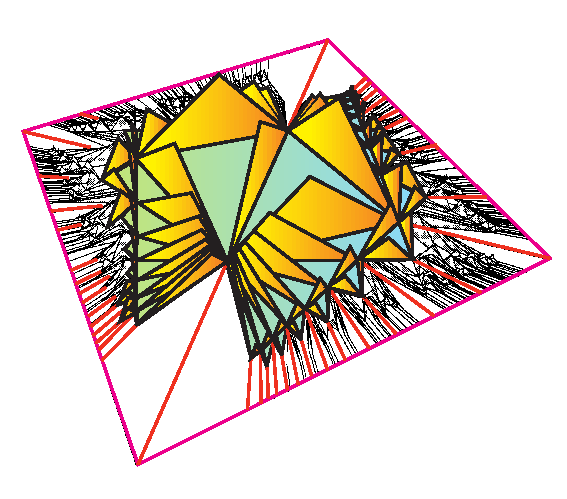
\includegraphics[width=\textwidth]{./Images/outerSpaceD2.pdf}
		\caption{Outer space $\mathcal{X}_{2}$}
	\end{subfigure}
	\hspace{0.1\textwidth}
	\begin{subfigure}{0.3\textwidth}
		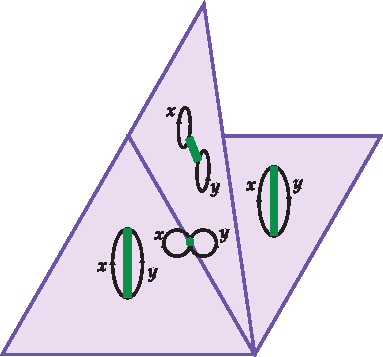
\includegraphics[width=\textwidth]{./Images/outerSpaceFaces.pdf}
		\caption{Simplices in $\mathcal{X}_{2}$}
	\end{subfigure}
\end{figure}

For a marked graph with $k+1$ edges, the corresponding simplex is $k$ dimensional.
Moreover, the identification works the other way round i.e. every open simplex in $X_{n}$ 
is a face of a maximal simplex that corresponds to a trivalent marked graph.
Taking the argument from the proof of Theorem \ref{thm:finGenCn} we see that the dimension of $\mathcal{X}_{n}$ is equal to $3n -4$.

Now with the Outer space defined we can consider the right group action of $\out(F_{n})$ on $\mathcal{X}_{n}$:
Every $\phi \in \out(F_{n})$ induces a map $f: R_{n} \to R_{n}$ by mapping the edge labelled
by $x$ to the edge labelled by $\phi(x)$.
Then the right group action is defined by $(g,G) \phi = (g \circ f, G)$.

An inconvenience that arises is that the quotient of $\mathcal{X}_{n}$ by $\out(F_{n})$ is not compact.
Resolving this leads us to the next construction.

\subsection{The spine of Outer space}
The beginning of this section follows Culler and Vogtmanns original definition from \cite{vogtmann86}.
In the latter half, we adhere to \cite{vogtmann16}.

In a first step, we define a more convenient and simpler version of $\mathcal{X}_{n}$ known as reduced Outer space and denote it by $Y_{n}$.
The points in the subspace $Y_{n}$ are the marked graphs $(g,G)$ that do not contain any separating edges, i.e.
no edges $e$ such that $G \setminus e$ is disconnected.
An equivariant deformation retraction from $\mathcal{X}_{n}$ to $Y_{n}$ is given by shrinking the lengths of
the separating edges to zero while uniformly extending the lengths of the other edges to preserve the total edge length of $1$.

We can now define the \emph{spine of Outer space} $K_{n}$ as follows:
$K_{n}$ is the maximal full\footnote{A subcomplex $B$ of a simplicial complex $A$ is said to be full if a simplex of $B$ all whose vertices are contained in $A$ is also a simplex of $A$.}
subcomplex of the barycentric subdivision of $Y_{n}$ which is disjoint from the boundaries of the open simplices in $Y_{n}$.
The vertices of $K_{n}$ are the barycenters of simplices in $Y_{n}$ i.e. the marked graphs whose edges are of equal length.
The deformation retraction from $Y_{n}$ to $K_{n}$ is given by
collapsing every simplex $\tau$ of the barycentric subdivision of $Y_{n}$ to the face of $\tau$ contained in $K_{n}$.
This can be done equivariantly.
Therefore $K_{n}$ can be thought of as ignoring the metric structure on $Y_{n}$ and only focusing on its combinatorial structure.

Going the other way if we have two vertices $(g,G)$ and $(g',G')$ in $K_{n}$. Then the open simplex in $\mathcal{X}_{n}$ 
determined by $(g,G)$ is a face of  the one determined by $(g',G')$ exactly when $G$ is obtained from $G'$ 
by collapsing a forest of edges in $G'$ and  $g$ is homotopic to the composition of $g'$ with the collapsing map.
This collapsing is also called a \emph{forest collapse}.
It follows that $K_{n}$ has the structure of a simplicial complex where a $k$-simplex is a chain of $k$ forest collapses. 

With this in mind we can determine the dimension of $K_{n}$: As collapsing an edge decreases the number of vertices by $1$
we see with a similar argument as in the proof of Theorem \ref{thm:finGenCn} that $\dim(K) = 2n -3$.
An example of a part of the spine of $\mathcal{X}_{2}$ is given in Figure \ref{fig:SpineOfXn}\footnote{This figure is taken from \cite{vogtmann02}}. 

\begin{figure}[h]
	\centering
	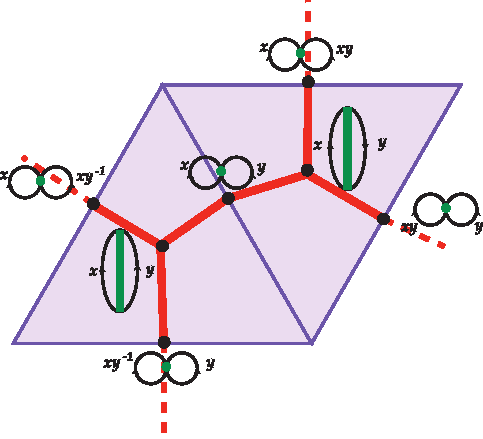
\includegraphics[width=0.3\textwidth]{./Images/spineOfOuterSpace.pdf}
	\caption{A section of the spine of Outer space $\mathcal{X}_{2}$.}
	\label{fig:SpineOfXn}
\end{figure}

Coming back to the right action of $\out(F_{n})$ on Outer space: This action on $\mathcal{X}_{n}$ extends to a simplicial action on $K_{n}$.
Culler and Vogtmann proved in \cite{vogtmann86} that this action has finite stabilizers.
Thus the rational homology of $\out(F_{n})$ can be computed as the quotient of $K_{n}$ by $\out(F_{n})$
\[
	H_{\bullet}(\out(F_{n}),\Q) \cong H_{\bullet}(K_{n}/ \out(F_{n}),\Q)
.\] 

To calculate this homology, we turn $K_{n}$ into a cube complex i.e. a CW complex where the cells are homeomorphic
to Euclidean cubes and the attaching maps identify faces with lower-dimensional cubes via homeomorphisms.
For a forest $\Phi$ in $G$ with $k$ edges we can now define the $k$-cube:
From $\Phi$ we get a chain of $k$-forest collapses by collapsing each edge in $\Phi$ at a time.
This yields a $k$-simplex. Collapsing the edges in another order yields another $k$-simplex.
All these different $k$-simplices can now be fit together to triangulate a $k$-dimensional cube.
Thus every $k$-cube is given by a graph $G$ and a forest $\Phi$ of size $k$.
The faces of dimension $k-1$ are the graphs obtained from $G$ where one edge in $\Phi$ has been collapsed.
An example is shown in Figure \ref{fig:spineCube}. Here the orange edges represent the edges that are being contracted along that face.

\begin{figure}[htbp]
	\centering
	\tikzfig{./tikzit/spineCube}
	\caption{A cube in the spine $K_{3}$}
	\label{fig:spineCube}
\end{figure}
Let us now view $K_{n}$ as this cube complex with one cube for every tuple $(g,G,\Phi)$. 
Then we can define an orientation on the cube via ordering the edges of $\Phi$ such that odd permutations reserve the orientation. 
Then the rational homology of $K_{n} / \out(F_{n})$ can be computed from a chain complex with one generator for each pair $(G,\Phi)$ that has no orientation
reversing-automorphism.

\subsection{The Forested graph complex}

The chain complex of pairs $(G,\Phi)$ computing $H_{k}(K_{n} / \out(F_{n});\Q)$ is generally known as the forested graph complex and has been
introduced by Conant and Vogtmann in \cite{conant03}. In this introductory section,
we will describe the original construction. In the later chapter, we are going to
introduce a more practical hands-on but equivalent definition from \cite{conant08}.

\begin{definition}
	A \emph{forested graph} is a pair $(G,\Phi)$ of a finite connected trivalent graph $G$ and an oriented forest $\Phi$ containing all vertices of $G$.
	The orientation on the forest is given by an ordering of its edges where interchanging any two edges reverses the orientation.
\end{definition}

We now denote by $\widehat{f\mathcal{G}}_{k}$ the vector space spanned by forested graphs with forest size $k$ modulo the relations
$(G,\Phi) = -(G,-\Phi)$.

If we consider a forested graph $(G,\Phi)$ and we collapse an edge $e$ in $\Phi$ then the obtained graph $(G_{e},\Phi_{e})$ 
has exactly one $4$-valent vertex. As the image below shows, there are exactly two other graphs
whose edge collapse leads to the graph $(G_{e},\Phi_{e})$.

\begin{figure}[bh]
	\centering
	\captionsetup{width=0.8\textwidth}
	\tikzfig{./tikzit/IHXRelator}
	\caption{The numbers represent the four parts of the graph that get connected at $e$.
		The graphs $G,G',G''$ then represent the three different ways how this can happen so that
	collapsing $e$ leads to $G_{e}$.}
\end{figure}

If we denote those two by $(G',\Phi')$ and  $(G'',\Phi'')$ then we call the vector
\[
	(G,\Phi) + (G',\Phi') + (G'',\Phi'')
.\] 
the basic IHX relator associated to $(G,\Phi,e)$. 
We denote by $IHX_{k}$ the subspace of $\widehat{f\mathcal{G}}_{k}$ spanned by all basic IHX relators
and define $f\mathcal{G}_{k}$ as the quotient space $\widehat{f\mathcal{G}}_{k} / IHX_{k}$.

Finally, we can define a boundary map  $\partial: f\mathcal{G}_{k} \to f\mathcal{G}_{k+1}$ induced by the map on $\widehat{f \mathcal{G}}_{k}$ given by
\[
	\partial_{E}(G,\Phi) = \sum (G,\Phi \cup e)
\] 
where we sum over all edges in $G \setminus \Phi$ such that $\Phi \cup e$ is still a forest and 
$e$ gets the label $k+1$ in the orientation.

One can check that $\partial_{E}$ is a boundary map that is $\partial_{E}^2 = 0$.
With this shown we get a chain complex $f\mathcal{G}_{\bullet}$ with boundary map $\partial_{E}$.
The rational homology of this complex computes the rational homology of $\out(F_{n})$ as
explained at the end of the previous section.

\subsection{The known homology of \texorpdfstring{\boldmath$\out(F_{n})$}{Out(Fn)}}
To conclude this introduction we try to summarize the known rational homology of $\out(F_{n})$.
As we only consider the rational homology, we will omit the field $\Q$.

For this we need to first introduce two concepts:
\begin{definition}
	If a group $G$ contains a torsion-free subgroup of finite index, then the \emph{virtual cohomological dimension} $\on{vcd}(G)$
is the cohomological dimension of this subgroup. It is independent of the choice of subgroup.

Moreover, a series of groups $G_1 \subseteq G_2 \subseteq \ldots$ is called \emph{homologically stable} if for every $k$ 
there exists a $N$ such that 
\[
	H_{k}(G_{n}) \cong H_{k}(G_{n+1}) \qq{ for all } n \geq N
\]
that is for $n$ large enough the homology is independent of  $n$.
\end{definition}

Culler and Vogtmann showed in \cite{vogtmann86} that $H_{k}(\out(F_{n}))$ is finitely generated and vanishes for $k$ greater
than the vcd of $\out(F_{n})$ which is $2n -3$. This gives us an upper bound on homology.
Furthermore, they showed that the spine $K_{n}$ is path-connected from which we conclude that $H_0(\out(F_{n})) = \Q$.

On the other side homological stability was proven for $\out(F_{n})$ for $n \geq 5 (k+1) / 4$ in \cite{hatcher04,hatcher98}.
Galatius proved in \cite{galatius11} that these groups are in fact zero, giving us a lower bound.

Only five of the non-trivial homology groups are explicitly known.
For the groups $H_{4}(\out(F_{4}))$, $H_{8}(\out(F_{6}))$ and $H_{12}(\out(F_{8}))$ it is known 
that the Morita classes do not vanish and in fact as these homology groups have dimension $1$ they are generated by the Morita classes.
We will expand on this in chapter \ref{sec:MoritaClasses}.
Ohashi showed in \cite{ohashi08} that all other groups for $n \leq 6$ are trivial. 
The only other known groups were determined by Bartholdi in \cite{bartholdi16} and are
$H_{8}(\out(F_{7}))$ and $H_{11}(\out(F_{7}))$. He also showed that all other homologies for $n = 7$ are trivial.
Figure \ref{fig:homologyOfOutFn} has been adapted from Figure 1 in \cite{conant16} and summarizes these results.

\begin{figure}[htbp]
	\centering
	\captionsetup{width=0.9\textwidth}
	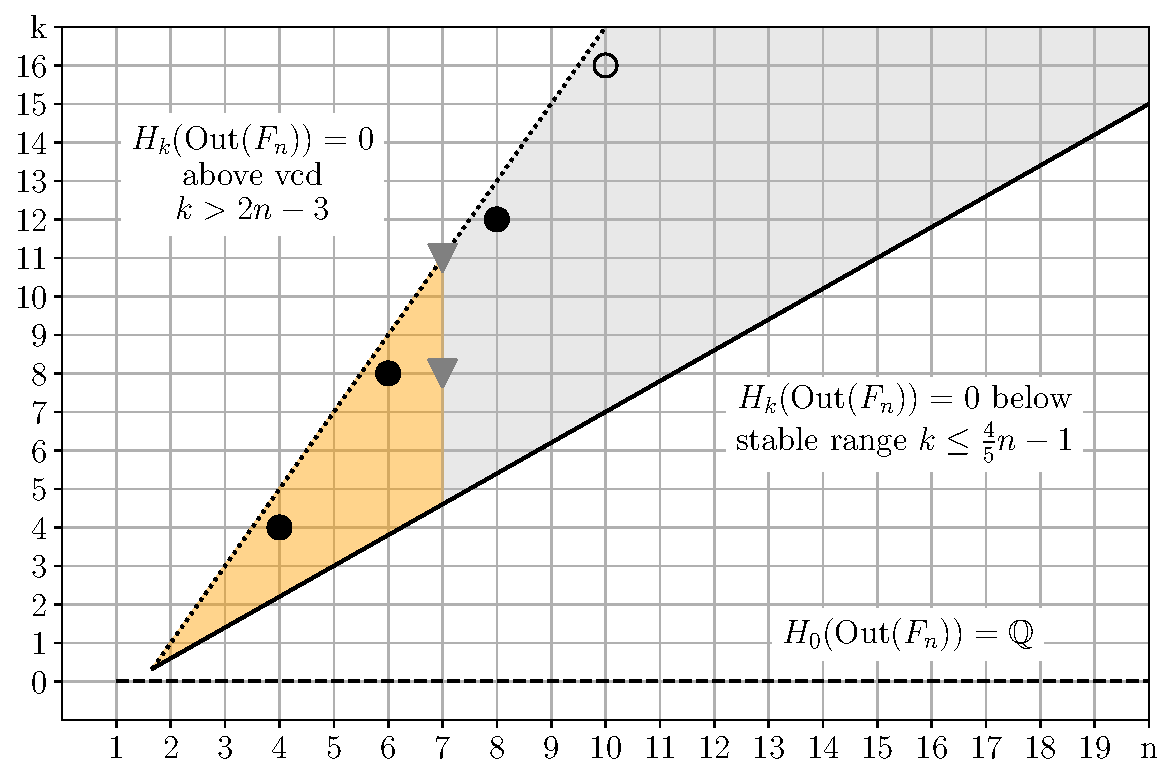
\includegraphics[width=0.9\textwidth]{./Images/OutFnHomology.pdf}
	\caption{Homology Classes of $\out(F_{n})$. The squares represent the  Morita classes and are filled in if they are known to be non-trivial.
		The hexagons are Bartholdi's non-trivial classes.}
	\label{fig:homologyOfOutFn}
\end{figure}

The Euler characteristic of a topological space is the alternating sum over the rank of the homology groups.
Computations of it for $\out(F_{n})$ were done by Morita, Sakasai and Suzuki in \cite{morita15moduli,morita15euler} for $n \leq 11$ and are shown in the table below.

\newcolumntype{C}{>{$}c<{$}}
\begin{table}[htpb]
	\centering
	\begin{tabular}{C|C|C|C|C|C|C|C|C|C|C}
		n & 3 & 4 & 5 & 6 & 7 & 8 & 9 & 10 & 11 & 12\\ \hline
		\chi(\out(F_{n})) & 1 & 2 & 1 & 2 & 1 & 1 & -21 & -124 & -1202 & ?
	\end{tabular}
\end{table}

The rapidly increasing negativity in the end implies that there are lots of odd-dimensional homology classes for $n$ equal to  $9,10,11$
and onward if this trend continues.
The only known odd-dimensional homology class however is Bartholdi's $H_{11}(\out(F_{7}))$.
Thus we see that the homology of $\out(F_{n})$ still remains mostly unknown.

\section{The forested graph complex}
Before we can introduce the forested graph complex we need a few more results about graphs.
\subsection{Further results on graphs}
\label{sec:RankGraph}
We begin this section by proving Theorem \ref{thm:fg_graph} which we state again below.
Afterwards, we expand on the concept of rank and prove several identities and relations.

\textbf{Theorem \ref{thm:fg_graph}.} \textit{Let $G$ be a graph. Then its fundamental group $\pi_{1}(G)$ is isomorphic to a free group.}

\begin{proof}
	The following proof is from \cite[p. 43f]{hatcher00}.
	Let $G$ be a graph. W.l.o.g. $G$ is connected as else we consider each connected component separately. 
	Let $T$ be a spanning tree on $G$ i.e. $T$ is a tree containing every vertex of $G$.

	Now choose for every $e_{\alpha} \in E(G) \setminus T$ an open neighborhood $A_{\alpha}$ of $T \cup e_{\alpha}$ that deformation retracts onto $T \cup e_{\alpha}$.
	The intersection of such $A_{\alpha}$ deformation retracts onto $T$ and is thus contractible. 
	Moreover, as $G$ is connected as a graph $A_{\alpha}$ and $T$ are path-connected.
	Now the $A_{\alpha}$ form an open cover of $G$ and as $T$ is simply connected by Van Kampen's theorem we get that $\pi_{1}(G) = *_{\alpha} \pi_{1}(A_{\alpha})$.
	Finally, $A_{\alpha}$ deformation retracts onto $S^{1}$ and thus $\pi_{1}(A_{\alpha}) = \Z$. Now there are exactly $\abs{E(G)} - \abs{E(T)}$ many $A_{\alpha}$,
	which as $T$ is a spanning tree and hence $\abs{E(T)} = \abs{V(G)}-1$ results in $\pi_1(G)$ being free on $\abs{E(G)} - \abs{V(G)} + 1$ generators.
\end{proof}

To understand the rank better we will need the following definitions
\begin{definition}
	For a finite CW complex $X$ the \emph{Euler characteristic} is defined as the alternating sum
	\[
		\chi(X) = k_0 - k_1 + k_2 - \ldots
	\] 
	where $k_{i}$ denotes the number of cells of dimension $i$ in the CW complex $X$.
\end{definition}
As graphs are $1$-dimensional we thus get $\chi (G) = k_0 - k_1$ which is equal to $\chi(G) = \abs{V(G)} - \abs{E(G)}$.

\begin{definition}
	Let $G$ be a graph. Then its \emph{cycle space} is the set of even-degree subgraphs of $G$ i.e. the subgraphs of $G$ whose vertices have even degree. 
	This space forms a vector space over $\F_2$ where the vector addition is given by the symmetric difference of two or more subgraphs.
	A basis of this space is called \emph{cycle basis} and two cycles are \emph{independent} if they are linearly independent in the vector space.
\end{definition}

\begin{remark}
	The cycle space is equal to the first homology group of $G$ with coefficients in $\F_2$ i.e. $H_1(G,\F_2)$.
\end{remark}

The following proposition relates the rank to different invariants and gives an easy way to compute it: 
\begin{proposition}\label{prop:rank}
	Let $G$ be a connected graph. Then the following are equal:
	\begin{enumerate}
		\item The rank of $G$.
		\item The number of independent cycles in $G$ i.e. the size of the cycle basis of $G$.
		\item The first Betti number i.e. the rank of $H_{1}(G)$.
		\item $1 - \chi(G) = \abs{E(G)} - \abs{V(G)} + 1$.
	\end{enumerate}
\end{proposition}

For the proof we will need the following lemma:
\begin{lemma}
	Let $A$ be a set. Then the abelianization of the free group on $A$ is isomorphic to the free abelian group on $A$.
\end{lemma}

\begin{proof}
	Consider the space $X = \bigvee_{a \in A} S^{1}$. By Van Kampen's theorem $\pi_1(X) \cong *_{a \in A} \Z$ that is $\pi_1(X)$ is isomorphic to the free group on $A$.
	Conversely, we have $H_1(X) \cong \bigoplus_{a \in A} H_1(S_1) \cong \bigoplus_{a \in A} \Z$ that is $H_1(X)$ is isomorphic to the free abelian group on $A$, 
	which follows from the relative homeomorphism theorem.
	Now using Hurewicz theorem we get that the abelianization of $\pi_1(X)$ is isomorphic to $H_1(X)$ and thus the desired statement.
\end{proof}

\begin{proof}[Proof of the Theorem]
	(1) = (4): This was shown in the proof of Theorem \ref{thm:fg_graph}.\\
	(1) = (3): From Hurewicz Theorem we get that the abelianization of $\pi_{1}(G)$ is equal to $H_{1}(G)$
	and thus by the previous Lemma that the rank of $\pi_1(G)$ is equal to the rank of $H_1(G)$ which is the first Betti number.\\
	(4) = (2)\footnote{This proof is based on Harary's proof in \cite[p. 37-40]{harary69}.}:
		Consider again the sets $A_{\alpha}$ from the proof of Theorem \ref{thm:fg_graph}. Each of them deformation retracts onto a cycle in $G$.
	Let $Z(T)$ be the set of cycles obtained in this way. Then  $Z(T)$ is independent as each cycle contains an edge not contained in any other cycle.
	Moreover, every cycle $Z$ in $G$ can be written as the symmetric difference over the cycles corresponding to the edges in $(E(G) \setminus T) \cap Z$.
	Thus $Z(T)$ spans the cycle space and consequently is a cycle basis. Now the size of $Z(T)$ is given by $\abs{E(G)} - \abs{V(G)} + 1$ and thus we conclude.
\end{proof}

Finally, we introduce the notion of the degree of a graph also sometimes called excess.
\begin{definition}
	Let $G$ be a connected graph of rank $n$ with vertex-valency $\geq 3$. Its \emph{degree} is defined by
	\[
		\deg(G) := \sum_{v \in V(G)} (\deg(v) - 3)
	.\] 
\end{definition}

\begin{proposition}
	Let $G = (V,E)$ be a graph of rank $n$. Then we have the following identities:
	\begin{enumerate}
		\item $\deg(G) = 2 \abs{E} - 3 \abs{V}$
		\item $\abs{V} = 2n -2 - \deg(G)$
		\item $\abs{E} = 3n - 3 - \deg(G)$
		\item $G$ is $3$-regular $\Leftrightarrow \deg(G) = 0$.
	\end{enumerate}	
\end{proposition}

\begin{proof}
	By counting half edges we get $2 \abs{E} = \sum_{v \in V} \deg(V)$.
	Combining this with the definition of degree we directly get the first identity.
	Using Proposition \ref{prop:rank} and the first identity we have
	\begin{align*}
		2 n -2 - \deg(G) &= 2 \abs{E} - 2 \abs{V} + 2 - 2 - 2\abs{E} + 3 \abs{V} = \abs{V}\\
		3 n -3 - \deg(G) &= 3 \abs{E} - 3 \abs{V} + 3 - 3 - 2\abs{E} + 3 \abs{V} = \abs{E}
	\end{align*}
	which proves the second and third identities. The last statement follows as every element in the sum of the degree is non-negative.
	Thus $\deg(G) = 0$ if and only if every term is $0$ and thus if and only if every vertex has valency $3$.
\end{proof}

\subsection{Forested graphs and the boundary map}
As stated in the introduction, the forested graph complex has first been introduced by Conant and Vogtmann in \cite{conant03}.
Here however we will introduce the simplified construction and definition of the forested graph complex given by Conant and Vogtmann in \cite{conant08}.
Very useful in the general understanding of  what a graph complex is and how the boundary map acts was Bar-Natan's and McKay's draft \cite{natan01}.
Inspired by this similar examples for the forested graph complex are presented.

Let $F_{n}$ denote the free group of rank $n$. We also denote by $\mathbb{S}_{n}$ the symmetric group of degree $n$.
\begin{definition}
	An \emph{admissible graph of rank $n$} is a $2$-edge-connected graph $G$ with vertex-valency $\geq 3$ whose fundamental group is isomorphic to $F_{n}$.
\end{definition}

We often abbreviate an admissible graph of rank $n$ by a graph.

\begin{definition}
	Let $G = (V,E)$ be a graph. An \emph{ordering} on its edges is a bijective function $\sigma$ from $E$ to $\{1,\ldots,\abs{E(G)}\}$.
	Notice that $\mathbb{S}_{\abs{E}}$ acts on $\sigma$ by $\pi \circ \sigma$ for $\pi \in \mathbb{S}_{n}$.
	We call the tuple $(G,\sigma)$ an ordered graph and note that $\mathbb{S}_{\abs{E}}$ acts on $(G,\sigma)$ by $\pi (G,\sigma) = (G,\pi \sigma)$ for $\pi \in \mathbb{S}_{\abs{E}}$.

	A \emph{forested graph} is a triple $(G,\Phi,\sigma)$ where $G$ is an admissible graph $\Phi$ is a subset of edges that spans a forest on $G$ and 
	$\sigma$ is an ordering on $\Phi$ i.e. $\sigma : \Phi \to \{1,\ldots,\abs{\Phi}\}$.

	A map $f$ between two forested graphs $(G,\Phi, \sigma) \to (H,\Psi, \tau)$ is said to be a \emph{forested graph} isomorphism if 
	$f$ is a graph isomorphism on $G$,  $f(\Phi) = \Psi$ and $\sigma = \tau \circ f $
\end{definition}

We now want to construct the forested graph complex. For this we remember the notion of a graded vector space:
\begin{definition}
	A graded vector space, is a vector space $V$ and with a decomposition $\left(V_{n}\right)^{\infty}_{n=0} $ such that
	\[
		V = \bigoplus_{k=0}^{\infty} V_{k}
	.\] 
\end{definition}

We now consider the $\Q$-vector space $C$ spanned by isomorphism classes of forested graphs, subject to the relation
\[
	(G,\Phi, \pi \circ \sigma) = \sgn{\pi} \cdot (G,\Phi, \sigma) \qq{for all} \pi \in \mathbb{S}_{n}(\abs{\Phi})
.\]
Under this relation we call $\sigma$ an \emph{orientation}.
Observe that if $(G,\Phi, \sigma) \simeq (G,\Phi, \pi \circ \sigma)$ for an odd permutation $\pi$ then 
$(G,\Phi, \sigma) \simeq (G,\Phi, \pi \circ \sigma) = - (G,\Phi, \sigma)$ and thus $(G,\Phi, \sigma) = 0$ in  $C$.

We can define the following three gradings on $C$:
 \begin{itemize}
	\item Let $C^{n} \subseteq C$ be the subspace spanned by forested graphs of rank $n$. Then clearly  $C^{n} \cap C^{m} = \emptyset$ for $n \neq m$ and
		as every graph has a rank, we get that the $C^{n}$ form a grading on $C$.
	\item Let $C_{k} \subseteq C$ be the subspace spanned by forested graphs $(G,\Phi,\sigma)$ with $k = \abs{\Phi}$. Clearly, this also yields a decomposition of $C$ into a direct sum
		and thus gives another grading on $C$.
	\item Let  $C_{d} \subseteq C$ be the subspace spanned by forested graphs of degree $d$. Once again this yields a grading on $C$.
\end{itemize}
In the following, we will mostly be concerned with the first two gradings. In particular, we will consider the double-grading $C_{k}^{n}$,
where $k$ denotes the forest size and $n$ the rank. 

\begin{eg}\label{ex:fg}
	Consider the graphs $G, J$ from Example \ref{ex:gAuto}. Then $G$ and $J$ are admissible graphs of rank $4$ and $3$. Thus if we equip them with ordered forests 
	$(\Phi,\sigma), (\Psi,\tau)$ as below 
	(where the orange edges represent the forest and the numbers the orientation) we get forested graphs in $C^{4}_{4}$ and $C^{3}_{2}$ respectively.

	\ctikzfig{./tikzit/forested_graph_automorphism}

	Observe, that $(J,\Psi) = 0$ in $C_{2}^{3}$, since $ (1 2)$ is an odd permutation and  $(1 2) (J,\Psi)$ is isomorphic to $(J,\Psi)$ 
	via the isomorphism mirroring vertices along the vertical line passing through the vertices labelled $1$ and $4$.

	$(G,\Phi)$ however is not trivial as the automorphism group is given by the identity,
	mirroring along the vertical, exchanging inner and outer vertices and their composition.
	None of these automorphisms induce an odd permutation and hence $(G,\Phi)$ does not vanish.
\end{eg}

Before we construct the chain complex we show that the $C^{n}$ are finitely generated and thus so are the $C_{k}^{n}$.

\begin{theorem}\label{thm:finGenCn}
	For all $n$, $C^{n}$ is finitely generated and $C_{k}^{n} = 0$ for all $k > 2n-3$. 
\end{theorem}

To prove this theorem we first need the following lemma:
\begin{lemma}
	For $n,m \in \N$ There are only finitely many admissible graphs $G = (V,E)$ with $\abs{V} \leq n$ vertices and $ \abs{E} \leq m$ edges.
\end{lemma}

\begin{proof}
	Every graph on $n$ vertices can be written as incidence matrix and each entry is $\leq m$ if the graph has maximally $m$ edges. 
	Thus there are maximally $m^{n^2}$ many different incidence matrices for graphs with  $n$ vertices and maximally $m$ edges.
	As every graph corresponds to an incidence matrix this also gives an upper bound on the number of different graphs with $n$ vertices
	and maximally $m$ edges.

	Thus the maximal possible number of admissible graphs with $\leq n$ vertices and $\leq m$ edges is bounded by
	\[
		\sum_{k=1}^{n} m^{k^2} 
	\]
	which is finite.
\end{proof}

\begin{proof}[Proof of Theorem \ref{thm:finGenCn}]
	By counting half edges we have
	\[
		2 \abs{E} = \sum_{v \in V} \deg{v}
	.\] 
	Using that admissible graphs have vertex-valency $\geq 3$ and rearranging yields $\abs{E} \geq \frac{3}{2} \abs{V}$.
	From Proposition \ref{prop:rank} we get that $\abs{E} = \abs{V} + n-1$.
	Combining the two yields
	\[
		\abs{V} + n -1 \geq \frac{3}{2} \abs{V} \Leftrightarrow 2 (n-1) \geq \abs{V}
	\] 
	and plugging in the result in the identity from Proposition \ref{prop:rank} yields $\abs{E} \leq 3 (n-1)$.

	Thus by the above lemma, we have that there are only finitely many graphs with $\abs{V} \leq 2 (n-1)$ and $\abs{E} \leq 3(n-1)$.
	As each graph only has a finite number of forests and each of them has a finite number of orientations we get that
	$C^{n}$ is finitely generated.

	That $C_{k}^{n} = 0 \forall k > 2n -3$ follows from the bound on the number of vertices and the fact that a forest in a graph has maximally $\abs{V} - 1$ edges.
\end{proof}

\begin{remark}
	Notice that for $C^{n}$ to be finitely generated the constraint of vertex-valency $\geq 3$ in the definition of admissible graphs is necessary.
	As else we can consider the following family of graphs where the most left polygon is of arbitrary size:
	\ctikzfig{./tikzit/infinite_admissible_graphs}
	They all have rank $n$ (which can be checked via the Euler characteristic), are $2$-edge-connected and are not isomorphic as they have a different number of vertices/edges.
\end{remark}

\begin{remark}
	The bound on the $C_{k}^{n}$ can not be improved as the graph $J$ from the example above with the tree extended by the edge between the vertex labelled $1$ and $4$ has rank $3$ and
	tree size $3$ which equals $2 \cdot 3 -3$.
\end{remark}

To construct the forested graph complex we fix the rank $n$ and define the differential as follows:
\begin{definition}
	Let $(G,\Phi,\sigma) = (G, \{e_1,\ldots,e_{k}\},\sigma)$ be a forested graph. Then let $\partial_{C}, \partial_{R}: C_{k}^{n} \to C_{k-1}^{n}$ be given by
	\begin{align*}
		\partial_{C}(G,\Phi,\sigma) &= \sum_{i = 1}^{k} (-1)^{i} (G / e_{i}, \Phi \setminus \{e_{i}\}, \sigma_{e_{i}}),\\
		\partial _{R}(G,\Phi,\sigma) &= \sum_{i = 1}^{k} (-1)^{i} (G,\Phi \setminus \{e_{i}\}, \sigma_{e_{i}}) 
	\end{align*}
	where $\sigma_{e_{i}}: \Phi \setminus \{e_{i}\} \to \{1,\ldots,k-1\}$ is given by
	\[
		\sigma_{e_{i}}(e) = \begin{cases}
			\sigma(e) & \text{ if }\sigma(e) < i\\
			\sigma(e) - 1 & \text{ if } \sigma(e) > i
		\end{cases}
	.\]
	Notice that the case $\sigma(e) = i$ cannot happen as $e_{i}$ is not contained in $\Phi \setminus \{e_{i}\}$. 
	Finally define the boundary map $\partial := \partial_{C} - \partial_{R}$.
\end{definition}

\begin{proposition}
	$\partial$ is well-defined and $\partial^2 = 0$.
\end{proposition}

For better readability, we will omit the orientation $\sigma$ in the proof.
\begin{proof}


	We proof the result in three steps:\\
	\textbf{Step 1:} Contracting an edge of a graph does not change the Euler characteristic as both the vertex number and the edge number decrease by one.
	Thus $\partial_{C}$ preserves the rank of the graph. Moreover, the vertex-valency stays $\geq 3$ and the graph continues to be $2$-edge-connected.
	Hence it is admissible.
	Furthermore, $\partial_{C}$ as well as $\partial_{R}$ remove one edge from each forest. Thus decreasing
	$k$ by $1$. Hence both maps are well-defined from $C^{n}_{k}$ to $C^{n}_{k-1}$ and thus so is $\partial$.

	Let $(G,\Phi) \in C^{n}_{k}$ be a forested graph with $\Phi = \{e_1,\ldots,e_{k}\}$  and denote the edges in $\Phi \setminus \{e_{i}\}$ by $\{e_1',\ldots,e_{k-1}'\}$,
	where $e'_{j} = e_{j}$ for $j < i$ and $e'_{j} = e_{j+1}$ for $j > i$.
	For the consecutive steps we need the following observations:
	\[
		(G / e_{i}) /  e_{j}' = \begin{cases}
			(G / e_{j}) / e_{i-1}' & \text{ if } i > j\\
			(G / e_{j+1}) / e_{i}' & \text{ if } i \leq j
		\end{cases}
		\qq{ and }
		(\Phi \setminus \{e_{i}\}) \setminus \{e_{j}'\}  = \begin{cases}	
			(\Phi \setminus \{e_{j}\}) \setminus \{e_{i-1}'\} & \text{ if } i > j\\
			(\Phi \setminus \{e_{j+i}\}) \setminus \{e_{i}'\} & \text{ if } i \leq j
		\end{cases}
	\]

	\textbf{Step 2:} \emph{Claim:} $\partial_{C}^2 = 0$ and $\partial_{R}^2 = 0$

	We compute:
	\begin{align*}
		\partial_{C}^2 &= \partial_{C} \sum_{i=1}^{k} (-1)^{i}(G / e_{i}, \Phi \setminus \{e_{i}\})
		=  \sum_{i=1}^{k} \sum_{j=1}^{k-1} (-1)^{i+j}((G / e_{i}) / e_{j}', (\Phi \setminus \{e_{i}\} ) \setminus \{e_{j}'\})  \\
					   &= \sum_{j < i} (-1)^{i+j} ((G / e_{i}) / e_{j}', (\Phi \setminus \{e_{i}\} ) \setminus \{e_{j}'\}) + \sum_{i \leq j} (-1)^{i+j}
					   ((G / e_{i}) / e_{j}', (\Phi \setminus \{e_{i}\} ) \setminus \{e_{j}'\}) \tag{$\star$}
	\end{align*}
	We claim that the two sums cancel. For this first apply the observations above to the first sum and then change variables by setting $l = j$ and  $m = i-1$ to obtain:
	\begin{align*}
		\sum_{j < i} (-1)^{i+j} ((G / e_{i}) / e_{j}', (\Phi \setminus \{e_{i}\}) \setminus \{e_{j}'\} ) &= 
		\sum_{j < i} (-1)^{i+j}((G / e_{j}) / e_{i-1}', (\Phi \setminus \{e_{j}\}) \setminus \{e_{i-1}'\} ) \\ 
		&= \sum_{l \leq m} (-1)^{l+m+1} ((G / e_{l}) / e_{m}', (\Phi \setminus \{e_{l}\}) \setminus \{e_{m}'\} ) 
	\end{align*}
	This last expression is the same as the second sum in $(\star)$ but with opposite sign. Thus they cancel and we have shown $\partial_{C}^2 = 0$.
	The same argument shows that $\partial_{R}^2 = 0$.

	\textbf{Step 3:} \emph{Claim:} $\partial_{C} \partial_{R} - \partial_{R} \partial_{C} = 0$

	For the mixed terms, we compute as follows
	\begin{align*}
		\partial_{R} \partial_{C} &=  \sum_{i=1}^{k} \sum_{j=1}^{k-1} (-1)^{i+j}(G / e_{i}, (\Phi \setminus \{e_{i}\} ) \setminus \{e_{j}'\})  \\
					   &= \sum_{j < i} (-1)^{i+j} (G / e_{i}, (\Phi \setminus \{e_{i}\} ) \setminus \{e_{j}'\}) + \sum_{i \leq j} (-1)^{i+j}
					   (G / e_{i}, (\Phi \setminus \{e_{i}\} ) \setminus \{e_{j}'\}) \tag{$*$}
	\end{align*}
	and
	\begin{align*}
		\partial_{C} \partial_{R} &=  \sum_{i=1}^{k} \sum_{j=1}^{k-1} (-1)^{i+j}(G / e_{j}', (\Phi \setminus \{e_{i}\} ) \setminus \{e_{j}'\})  \\
					   &= \sum_{j < i} (-1)^{i+j} (G / e_{j}', (\Phi \setminus \{e_{i}\} ) \setminus \{e_{j}'\}) + \sum_{i \leq j} (-1)^{i+j}
					   (G / e_{j}', (\Phi \setminus \{e_{i}\} ) \setminus \{e_{j}'\}) \\
					   &\stackrel{(\heartsuit)}{=} \sum_{j < i} (-1)^{i+j} (G / e_{j}, (\Phi \setminus \{e_{j}\} ) \setminus \{e_{i-1}'\}) + \sum_{i \leq j} (-1)^{i+j}
					   (G / e_{j+1}, (\Phi \setminus \{e_{j+1}\} ) \setminus \{e_{i}'\}) \\
					   &\stackrel{(\dagger)}{=} \sum_{l \leq m} (-1)^{m+l+1} (G / e_{l}, (\Phi \setminus \{e_{l}\} ) \setminus \{e_{m}'\}) + \sum_{m < l} (-1)^{m+l-1}
					   (G / e_{l}, (\Phi \setminus \{e_{l}\} ) \setminus \{e_{m}'\}) \tag{$* *$}
	\end{align*}
	Where in $(\heartsuit)$ we used that if $j < i$ then $e_{j} = e_{j}'$ and if $i \leq j$ then $e_{j+1} = e_{j}'$, as well as the observation above.
	In $(\dagger)$ we used the substitution  $m = i-1$,  $l = j$ on the left and  $m = i$,  $l = j+1$ on the right sum.
	Comparing the sums in $(*)$ and $(* *)$ we see that they differ by a sign and thus cancel. Hence  $\partial_{C} \partial_{R} - \partial_{R} \partial_{C} = 0$.

	Combining Step 2 and 3 we get:
	\[
		\partial^2 = (\partial_{C} - \partial_{R})^2 = \partial_{C}^2 - (\partial_{C} \partial_{R} + \partial_{R} \partial_{C}) + \partial_{R}^2 = 0\qedhere
	\]
\end{proof}

Thus the spaces $(C^{n}_{\bullet})$ with the differential $\partial_{\bullet}$ form a chain complex.

\begin{eg}
	Once again we consider the graph $(G,\Phi)$ from Example \ref{ex:fg} and calculate its boundary operator:
	\ctikzfig{./tikzit/boundary_operator}
	Where we used that $-H_{1}$ is equal to $H_{2}$ by mirroring along the vertical and applying $(2 3)$,
	$-H_{3}$ is equal to $H_2$ by exchanging inner and outer vertices, mirroring along the vertical and applying $(1 3)$ and
	$H_{4}$ is equal to $H_{2}$ by exchanging inner and outer vertices and applying $(1 3)(2 3)$.
	Where we have used the permutation $(2 3)$ on the first,  $(1 3)$ on the third, $(1 3)(2 3)$ on the fourth graph to get the result.
	\ctikzfig{./tikzit/boundary_operator2}
	Where we have used that $-G_{1}$ is equal to $-G_{3}$ by exchanging inner and outer vertices and applying $(1 3)(1 2)$,
	$G_{2}$ is equal to $-G_{3}$ by exchanging, mirroring along the vertical and applying $(1 3)$ and
	$G_{4}$ is equal to $-G_{3}$ by mirroring along the vertical and applying $(1 2)$. 

	Thus we can conclude that $\partial_{\bullet} G = 4 H_2 - 4 G_3$. Moreover, we have that $H_2 - G_3 \in \im \partial_{\bullet}$ and 
	as $\partial_{\bullet}^2=0$ also $H_2 - G_3 \in \ker \partial_{\bullet}$
\end{eg}

\begin{remark}
As the example above shows these calculations, especially identifying isomorphic graphs and finding odd automorphisms, 
become quite tedious quickly. Therefore it is best to leave them to the computer and a python implementation
of this can be found in the appendix.
\end{remark}

Coming back to the forested graph complex $C^{n}$ it can be viewed as a cubical complex in a similar way to the spine of Outer space in the introduction:
The $k$-cubes are given by graphs $(G,\Phi,\sigma)$
with forest size $k$ and the faces are $k-1$-cubes obtained from collapsing an edge in $\Phi$ 
or removing an edge in $\Phi$ from the forest. Collapsing the edge $e \in \Phi$ is
on the opposite side of removing $e$ from $\Phi$ on the $k$-cube.
An orientation on the cube is induced by the signs from the boundary maps $\partial_{C}$ and $\partial_{R}$.

To visualize this construction we consider the following example:
\begin{eg}
	Consider again the graph $J$ from Example \ref{ex:gAuto} with the forest $\Phi$ given by an edge between the top and middle vertex and
	between the left and write vertex.
	Then its $2$-dimensional cube is given as below:
	\ctikzfig{./tikzit/cubicalCCEx}
\end{eg}
\newpage
\section{Morita cycles}\label{sec:MoritaClasses}
The goal of this section is to show that there exists a cycle in every $C^{m}_{2m-4}$.
For this we define the Morita graphs and show that there exists a chain of those graphs that vanishes under the boundary $\partial$.

\begin{definition}
	A \emph{Morita graph} $M_{n}(\sigma)$ for $n \in \N_{\geq 3}$, $\sigma \in \mathbb{S}_{n}$ is a forested graph $(G,\Phi,\tau)$ defined as follows:
	$G$ consists of two polygons with $n$ vertices, each of which is connected to precisely one vertex on the other polygon.
	The vertices are labelled from $1$ to $n$ on one polygon and $n+1$ to $2n$ on the other then the connecting edges between them are given by $(i,\sigma(i)+n)$ i.e.
	$\sigma$ describes how the edges connecting the two polygons are permuted.

	The forest $\Phi$ consists of the edges $(i,i+1)$ for $i \in \{1,\ldots,n-1, n+1,\ldots,2n-1\}$ i.e. the
	forest consists of two linear trees of size $n-1$ each of which is obtained by removing one edge from the corresponding polygon.
	Finally, the ordering $\tau$ is given by
	\[
		\tau((i,i+1)) = \begin{cases}
			i & \text{ for } 1 \leq i \leq n-1\\ 
			i-1 & \text{ for } n+1 \leq i \leq 2n-1
		\end{cases}
	.\] 
\end{definition}
Notice that for all even $n$ the graph $M_{n}(\sigma)$ has an odd automorphism which is given by exchanging the two polygons and applying the permutation $(1\ n) \ldots (n-1\ 2n -1)$.
Thus those Morita graphs vanish.
Moreover, as $M_{n}(\sigma)$ has $2n$ vertices and $3n$ edges by Proposition \ref{prop:rank} it has rank $n+1$.
Furthermore, $M_{n}(\sigma)$ is clearly an admissible graph and thus $M_{n}(\sigma) \in C^{n+1}$. Moreover as the forest size is $2n-2$ $M_{n}(\sigma)$ is in $C^{n+1}_{2n -2}$

To give a better understanding of this definition we give the following example:

\begin{eg}
	Below is a Morita graph of order $5$ given by the permutation $(12)(345)$.
	\ctikzfig{./tikzit/morita_cycle_5}
\end{eg}

The following result proves that there exists a cycle in every $C_{n}$ for $n \geq 4$.
\begin{theorem}
	For all $n \in \N_{\geq 3}$ odd it holds that 
	\[
		\partial\left(\sum_{\sigma \in S_{n}} \sgn(\sigma) M_{n}(\sigma)\right) = 0
	.\] 
	We call this sum a Morita cycle and denote it by $Z_{n}$
\end{theorem}

We prove this statement in two parts first for $\partial_{C}$ and then for $\partial_{R}$, from which the final result follows.


\begin{proof}[Proof for $\partial_C$]
	Let $(H,\Psi,\eta)$ be an element of the chain $\partial_{C} Z_{n}$.
	Then as it is an element of the boundary of some Morita graph it has to
	have precisely one vertex of degree $4$. W.l.o.g. we can assume that it is in the polygon containing the 
	edge with the label $1$ as else we can apply the even permutation $(1 \ldots 2n-1)^{n}$ to the orientation.

	Let $k$ be the label of the degree $4$ vertex. An example is shown in the figure below on the left for $k = 2$. 
	Then there exist exactly two Morita graphs in whose boundary $H$ lies and whose induced node labeling corresponds to the one of $H$.
	One is obtained by splitting the vertex $k$ into two vertices labeled $k$ and $k+1$ where each new vertex contains one edge from the forest and one connecting to the other polygon.
	Moreover, the two new nodes get connected by an edge which is also added to the forest and given the number $k$ in the ordering.
	All other edges with ordering number  $> k $ get their ordering number increased by one. Let us denote this Morita graph by $M_{n}(\sigma)$.
	The other one is obtained in the same way however the two edges connecting to the other polygon are permuted i.e.
	this Morita graph equals $M_{n}((k\ k+1)\sigma)$.
	Examples for both are also shown in the figure below in the middle and right respectively.

	Finally, we see that the two permutations $\sigma$ and $(k\ k+1) \sigma$ have opposite parity and thus $M_{n}(\sigma)$ and $M_{n}((k\ k+1) \sigma)$ have
	opposite signs in $Z_{n}$. Thus the elements in their boundary corresponding to $H$ also have opposite signs and hence cancel.

	As $H$ was an arbitrary element of $Z_{n}$ we get that every summand has coefficient $0$ and that $Z_{n}$ vanishes.
	\ctikzfig{./tikzit/morita_cycle_dC}
\end{proof}

\begin{proof}[Proof for $\partial_{R}$]
	Again let $(H,\Psi,\eta)$ be an element of the chain $\partial_{R} Z_{n}$.
	Then $H$ is a Morita graph whose forest $\Psi$ is missing one edge in one of its trees.
	We denote by $\sigma$ the edge permutation of $H$ between its two polygons as given in the definition of Morita graphs.
	W.l.o.g. we can assume that the tree with the missing edge contains the 
	edge with the label $1$ as else we can apply the even permutation $(1 \ldots 2n-1)^{n}$ to the orientation.
	
	Let $(j,j+1)$ denote the extra edge missing from  $\Phi$. An example is shown in the figure below on the left for $j = 2$.
	Then there are exactly two Morita graphs in the sum which have $H$ in their boundary and whose induced node labelling corresponds to the one of $H$.

	One where the edge $(j,j+1)$ has been given the number $j$ in the ordering, been added to the forest and later edges have gotten their numbering increased by $1$
	i.e. $M_{n}(\sigma)$.
	And the other where the edge $(1,n-1)$ has been added and the ordering is given by
	\[
		\tau((i,i+1)) = \begin{cases}
			i-j & \text{ for } j+1 \leq i \leq n-1\\
			n-j+i & \text{ for } 1 \leq i \leq j-1\\
			i-1 & \text{ for } n+1 \leq i \leq 2n-1
		\end{cases} \qq{and} \tau(1,n-1) = n-j
	\] i.e. the numbering starts with $1$ at the edge $(j+1,j)$ and increases until it reaches $n-1$ on the edge  $(j-1,j)$. 
	The ordering on the other polygon has not been altered.
	
	Notice that the second graph is not part of $Z_{n}$ as the node labelling and the forest ordering do not correspond anymore. 
	To resolve this we have to change the node labelling which induces the permutation $(1 \ldots n)^{k}$ on $\sigma$.
	Thus the element in the sum corresponding to this graph is given by  $M_{n}(\tau) := M_{n}(\sigma (1 \ldots n)^{k})$.
	Examples for both are also shown in the figure below in the middle and right respectively.
	As $(1 \ldots n)$ for $n$ odd has even parity $\tau$ and $\sigma$ have the same parity and thus $M_{n}(\tau)$ and $M_{n}(\sigma)$ have the same sign
	in the sum. 
	
	Finally taking the boundary the elements corresponding to $H$ have different orientations.
	The element in $\partial_{R}(M_{n}(\sigma))$ is exactly $H$ with sign $(-1)^{k}$. The element in $\partial_{R}(M_{n}(\tau))$ has sign $(-1)^{n-k}$ however, it 
	differs from $H$ by the permutation $(1 \ldots n-2)^{k - 1}$ with even parity as $n-2$ is odd.
	Now for $n$ odd if $k$ is even $n-k$ is odd and vice versa. Thus the elements corresponding to $H$ have opposite signs and cancel.

	As $H$ was an arbitrary element of $Z_{n}$ we get that every summand has coefficient $0$ and that $Z_{n}$ vanishes.

	\ctikzfig{./tikzit/morita_cycle_dR}

	Thus we have shown the result for both $\partial_{C}$ and $\partial_{R}$ and as $\partial = \partial_{C} - \partial_{R}$ it also follows that $\partial Z_{n} = 0$.
\end{proof}

\begin{remark}
	The Morita graphs are also included in the python implementation in the appendix and the above formula can be checked for small $n$.
	For $n=3$ and $n=5$ explicit isomorphism-reduced representations of the Morita cycles $Z_{n}$ can be seen in Figure \ref{fig:Z3} and \ref{fig:Z5} respectively.
	For larger $n$ these calculations becomes difficult very quickly as the number of Morita graphs is proportional to $n!$.
\end{remark}

\begin{figure}[h]
	\centering
	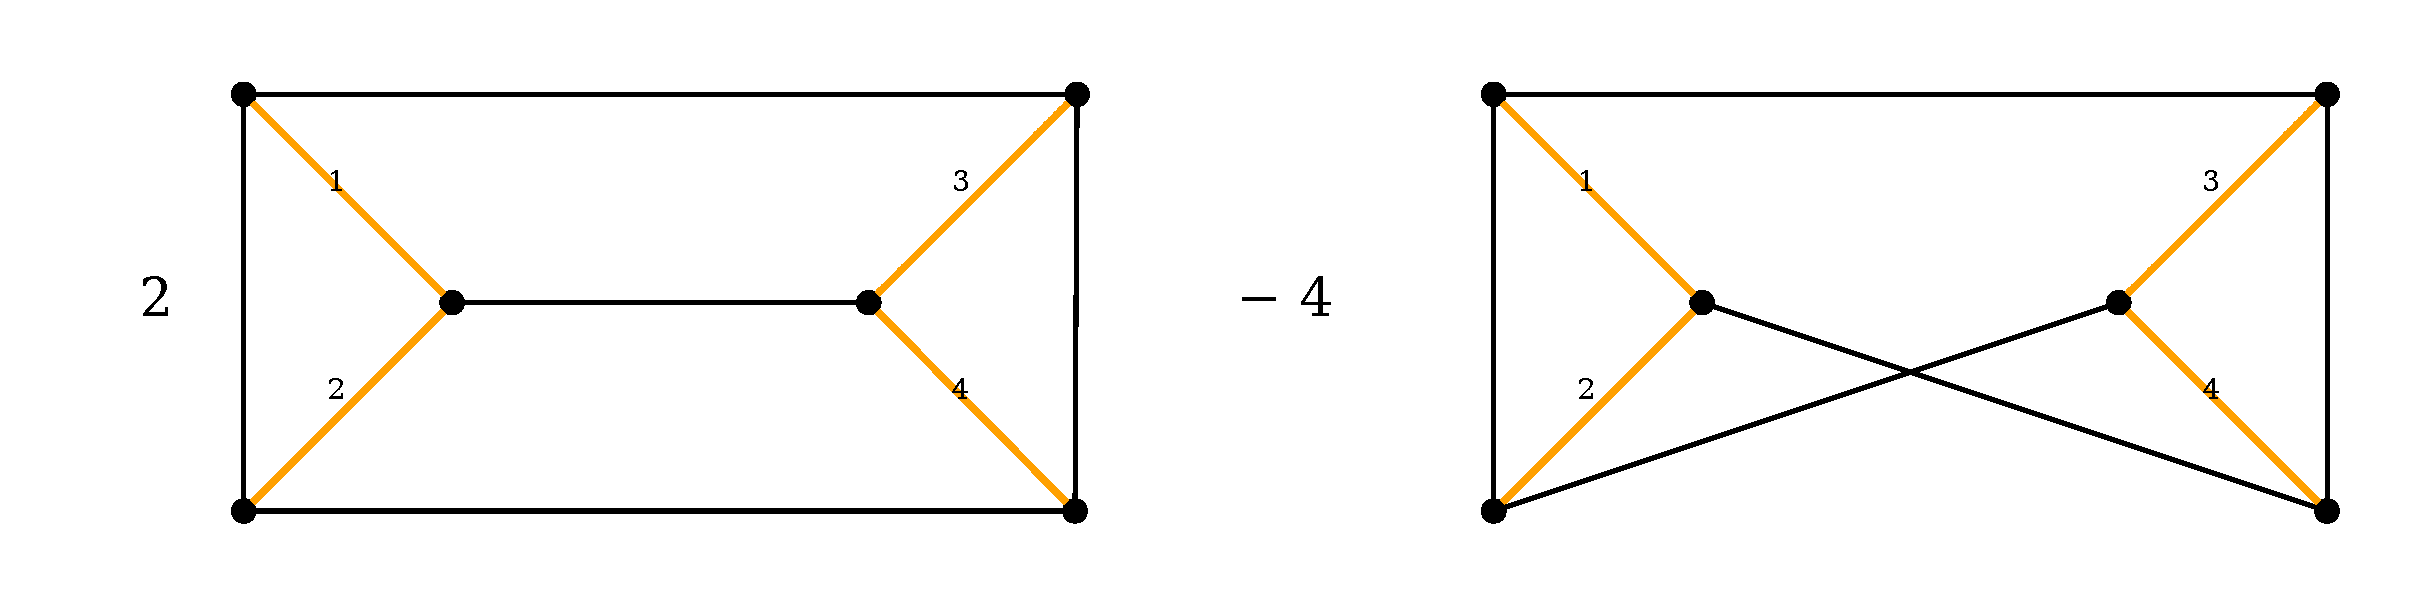
\includegraphics[width=\textwidth]{./ForestedGraphs/MCCycle3.pdf}
	\caption{Isomorphism reduced version of $Z_3$}
	\label{fig:Z3}
\end{figure}
\begin{figure}[p]
	\centering
	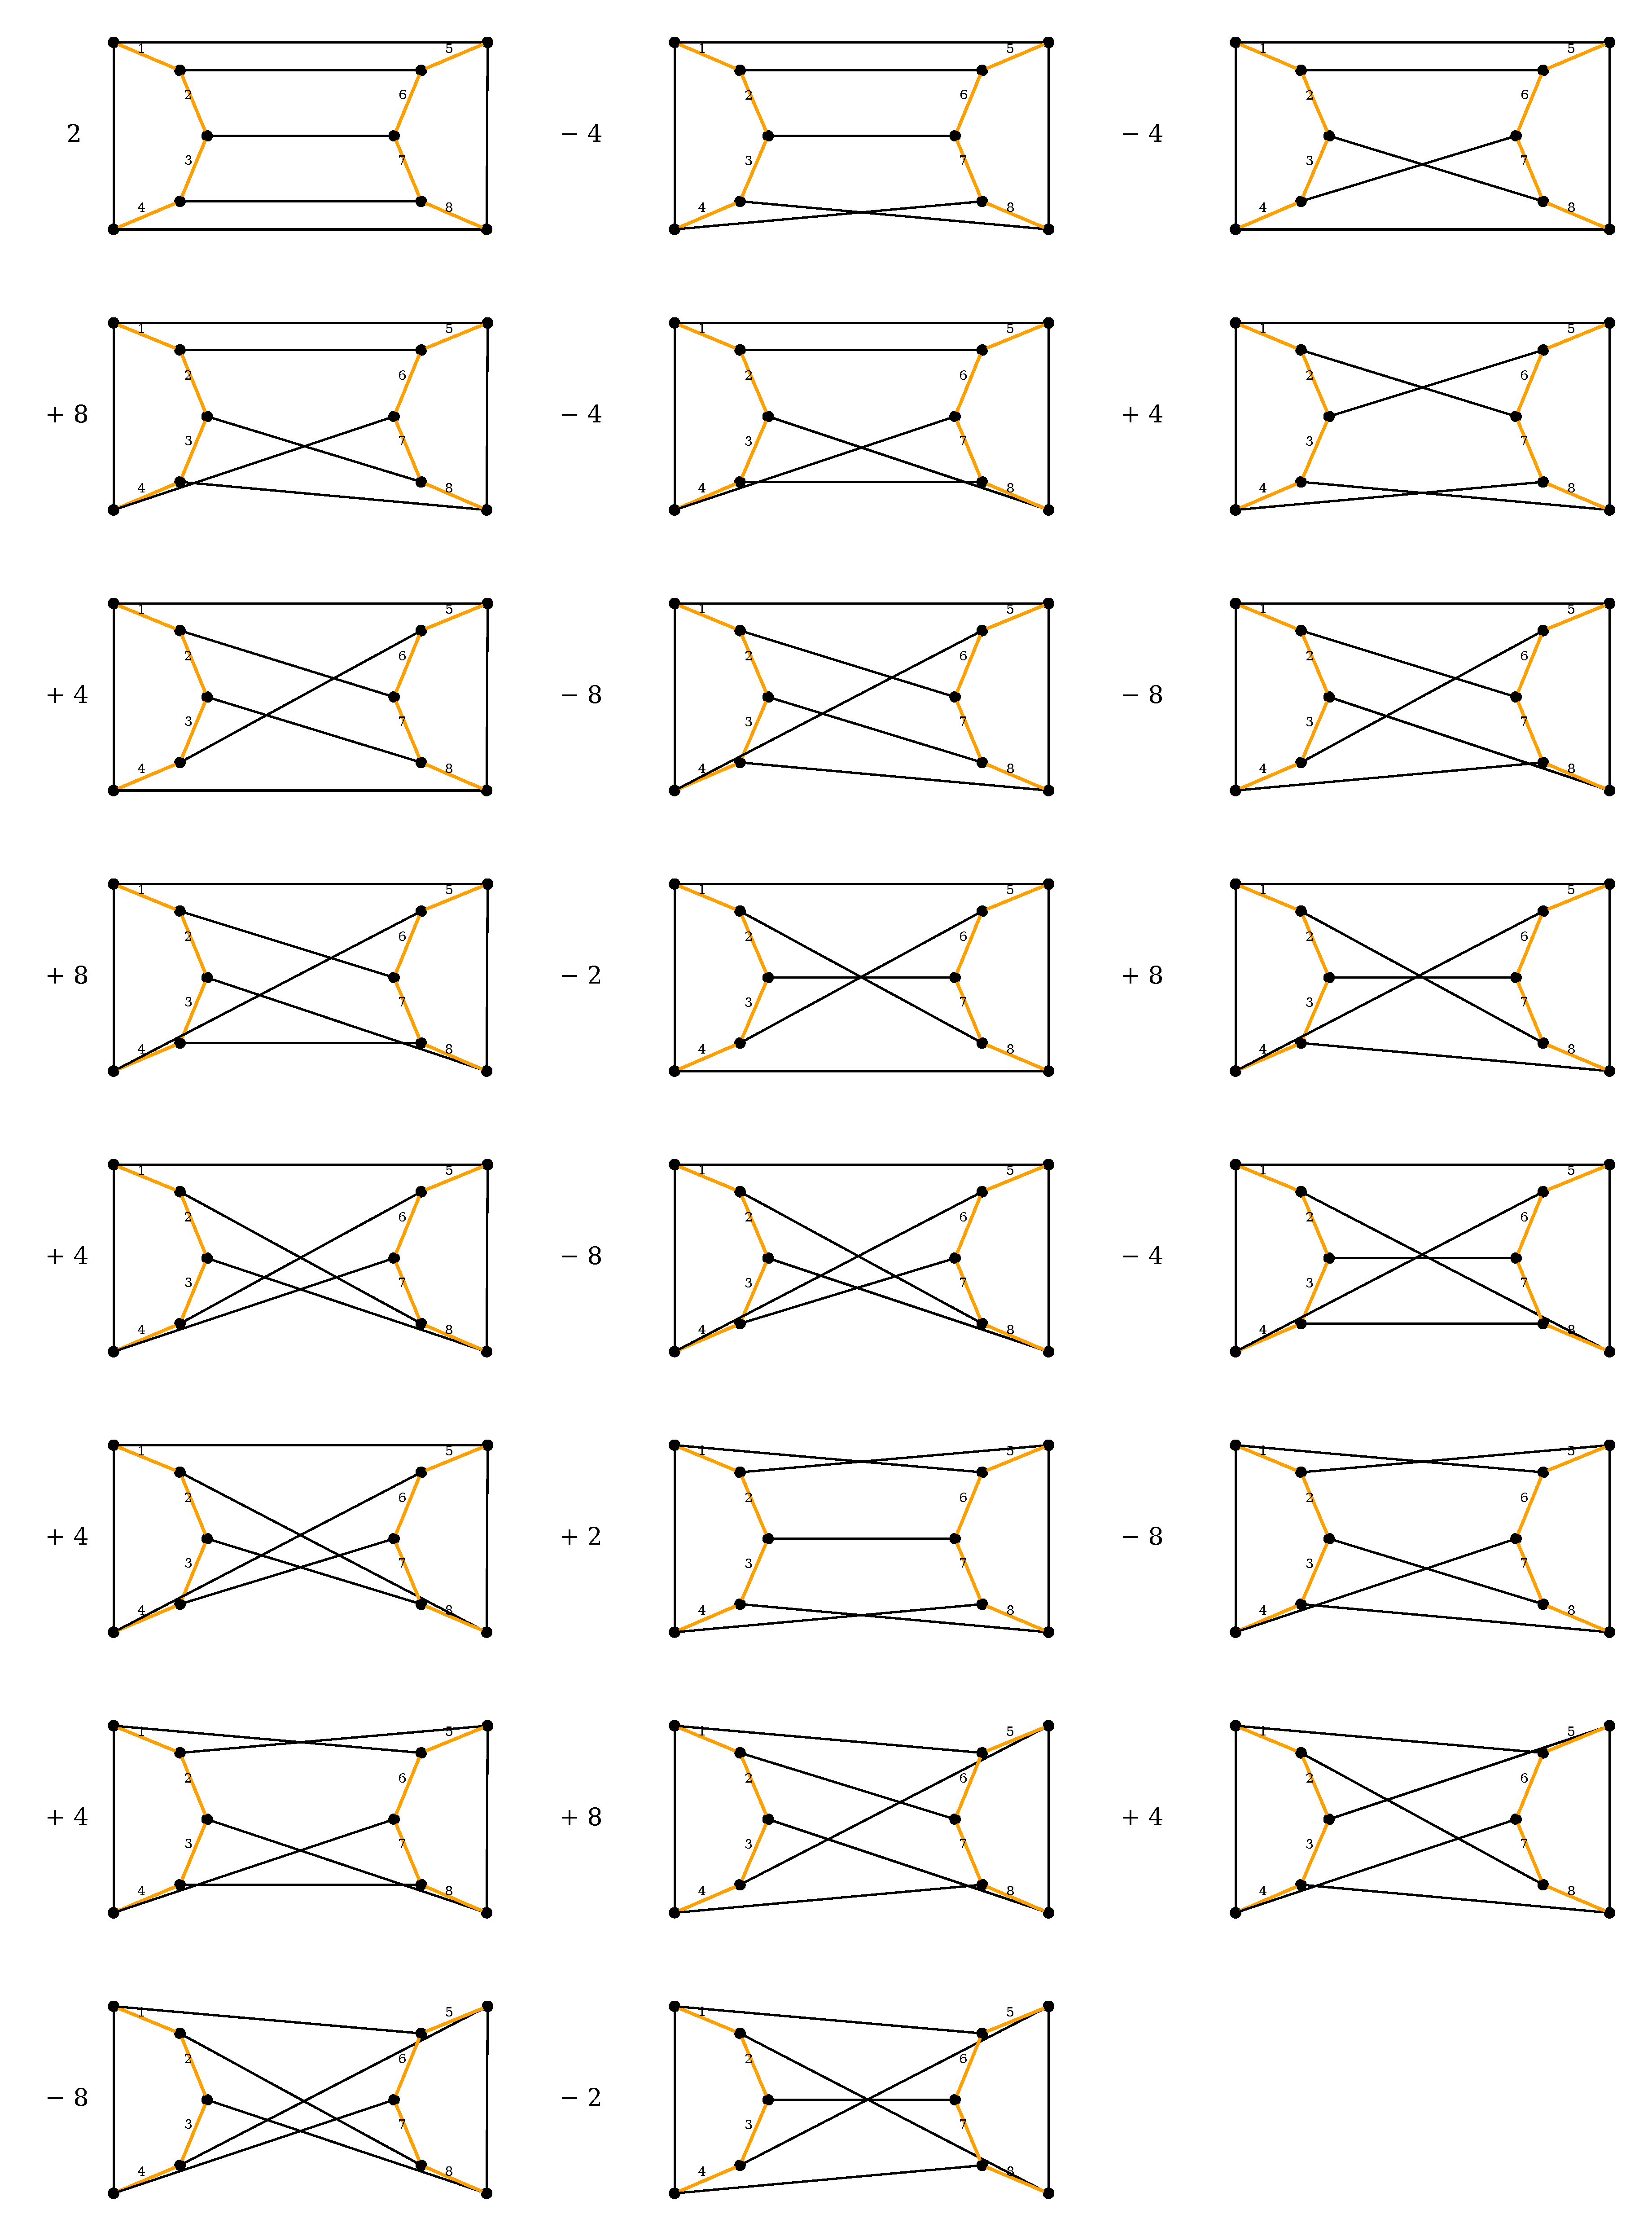
\includegraphics[width=\textwidth]{./ForestedGraphs/MCCycle5.pdf}
	\caption{Isomorphism reduced version of $Z_5$}
	\label{fig:Z5}
\end{figure}

A more general result, showing that a similar sum vanishes for $n$ polygons instead of just two,
has been shown by Conant and Vogtmann in \cite{conant08}.

As we have shown that these Morita cycles vanish under the boundary the question arises if they are
non-trivial in homology i.e. if they lie in the image of $\partial$ or not. 
Morita showed himself that the first cycle ($n=3$) is non-trivial and conjectured that 
all of his classes are non-trivial. Conant and Vogtmann showed in \cite{conant04} that 
the second cycle ($n=5$) is also non-trivial, Gray extended this
to show in \cite{gray11} that the third cycle ($n=7$ ) is non-trivial.
Both of these calculations relied partly on computer calculations
which increase extremely quickly with $n$. Thus Morita's conjecture
remains a challenging open problem to this day.

\newpage
\printbibliography
\newpage
\appendix
\section{Python implementation}
To run the ensuing code graphviz, a version of python 3 as well as the following packages are needed:
\begin{itemize}
	\item numpy
	\item sympy
	\item pydot
	\item networkx
\end{itemize}
The code consists of four files.
In the \texttt{boundaries.py} file $\partial_{C}$,$\partial_{R}$, $\partial$ as well as
the reduction up to isomorphisms and the vanishing of graphs with odd automorphisms is implemented.
The file \texttt{plotting.py} includes functions for plotting a single forested graph as well as a chain.
In \texttt{MoritaCycles.py} the generation of Morita graphs $M_{n}(\sigma)$ as well as
Morita cycles $Z_{n}$ and producing positions for plotting is realized.
Finally, in \texttt{main.py} a small working example reducing and plotting $Z_{n}$ as well as calculating
its boundary and printing it has been implemented.

\subsection{main.py}
\lstinputlisting[language=Python]{./ForestedGraphs/main.py}
\subsection{boundaries.py}
\lstinputlisting[language=Python]{./ForestedGraphs/boundaries.py}
\subsection{plotting.py}
\lstinputlisting[language=Python]{./ForestedGraphs/plotting.py}
\subsection{MoritaCycles.py}
\lstinputlisting[language=Python]{./ForestedGraphs/MoritaCycles.py}

%%\input{../header}

\section{Draftparts}

\begin{definition}
	A \emph{graph} $G$ is a finite $1$-dimensional CW complex. The set of edges is denoted by $E(G)$, the set of vertices by  $V(G)$ and the set of half edges by  $H(G)$.
	We call a graph \emph{connected} if the CW complex is connected in the topological sense.
	A graph is said to be \emph{$n$-valent} if every vertex has valency $n$ i.e. for every vertex the number of edges incident is  $n$.

	Lastly a \emph{tree} is a graph which contains no loops and a \emph{forest} is a collection of disjoint trees.
\end{definition}

On trivalent connected graphs we call an \emph{orientation} a choice of cyclic orders of all vertices up to an even number of changes.

\begin{definition}
	A \emph{forested graph} is a pair $(G, \Phi)$, where $G$ is a finite connected trivalent graph and $\Phi$ is an oriented forest which contains all vertices of $G$. 
\end{definition}

\begin{definition}
Let $(G,\Phi)$ be a forested graph and let  $e \in \Phi$. Moreover let $(G_{e},\Phi_{e})$ be the graph where $e$ has been collapsed.
Then there exist exactly two other graphs whose edge collapse results in $(G_{e},\Phi_{e})$. This is visualised in the figure below.
Where  $1,2,3,4$ represent the rest of the graph.

\ctikzfig{./tikzit/IHXRelator}
Now the vector 
\[
	(G,\Phi) + (G',\Phi') + (G'',\Phi'')
\]
is called the \emph{basic IHX relator} associated to $(G,\Phi,e)$.
\end{definition}

Denote by $\widehat{\fg}_{k}$ the vector space spanned by all forested graphs containing $k$ trees modulo the relations $(G,\Phi) = -(G,-\Phi)$.
Moreover let $\fg_{k}$ be the quotient of $\widehat{\fg}_{k}$ modulo the subspace spanned by all basic IHX relators.


\begin{definition}
	Let $\widehat{\partial}_E(G,\Phi): \widehat{\fg}_{k} \to \widehat{\fg}_{k-1}$ be given by
\begin{align*}
	\widehat{\partial}_{E}(G,\Phi) = \sum (G, \Phi \cup e)
.\end{align*}
where the sum is over all edges $e$ of $G \setminus \Phi$ such that $\Phi \cup e$ is still a forest.
Notice that this only happens if the two vertices of  $e$ lie in different trees of $\Phi$. Thus $\Phi \cup e$ has $k-1$ components.
The orientation of $\Phi \cup e$ is determined by ordering the edges of $\Phi$ with labels  $1,\ldots,k$ consistent with its orientation
and then labeling the new edge $e$ with  $k+1$.

Now let the boundary map $\partial_{E}: \fg_{k} \to \fg_{k-1}$ be the map induced by $p \circ \widehat{\partial}_{E}$ where $p$ is the quotient map $\widehat{\fg_{k}} \to \fg_{k}$.
\end{definition}

\begin{proposition}
	$\partial_{E}$ is well-defined and $\partial_{E}^2 = 0$.
\end{proposition}

\begin{proof}
	
\end{proof}

The \emph{forested graph complex} is thus defined as the sequence $\fg_{k}$ with boundary map $\partial_{E}$ and is well-defined by the above proposition.

\subsection{The Outer space}
We closely follow Vogtmann's definition from \cite[p. 2 ff.]{vogtmann16}
\begin{definition}
	By a \emph{metric graph} we mean a finite connected graph with positive real edge lengths, equipped with the path metric.
	We fix a model rose $R_{n}$ (a graph with one vertex and $n$ petals), and identify the petals of $R_{n}$ with the generators
	of the free group $F_{n}$. A point in $\mathcal{X}_{n}$ is then a metric graph $G$ together with a homotopy
	equivalence $g: R_{n} \to  G$ called a \emph{marking}; the marking serves to identify the fundamental group of $G$ with $F_{n}$.
	Marked graphs $(g,G)$ and $(g',G')$ are considered the same if there is an isometry  $f: G \to G'$ with $f \circ g$ homotopic to $g'$.

	To get a finite dimensional space we assume $G$ has no uni- and bivalent vertices (see Theorem \ref{thm:finGenCn}).
	Moreover we normalize our objects i.e. we assume the sum of edge lengths to be $1$ and assume that $G$ is $2$-connected.
\end{definition}
To make  $\mathcal{X}_{n}$ a space we need to define a topology. We proceed as follows: 
For every marked graph $(g,G)$ we define the open simplex $\sigma(g,G)$ as the set obtained by varying the edge lengths of $G$,
keeping their sum equal to $1$.
The simplex  $\sigma(g',G')$ is then a \emph{face} of $\sigma(g,G)$ if $(g',G')$ can be obtained from $(g,G)$ by collapsing some edges to points.

Finally $\mathcal{X}_{n}$ is the quotient space obtained from the disjoint union of the open simplices $\sigma(g,G)$ by face identification.

However not all faces of these simplices are in $\mathcal{X}_{n}$.
To rectify this we replace each open simplex $\sigma(g,G)$ by a closed simplex $\overline{\sigma}(g,G)$ and take
the quotient as before. This new space, denoted by $\mathcal{X}^{*}_{n}$, is a simplical complex and called the \emph{simplical closure} of Outer space.
The points in $\mathcal{X}^{*}_{n}$ which are not in $\mathcal{X}_{n}$ are said to be at infinity.

 Now the group $\out(F_{n})$ acts on $\mathcal{X}_{n}$ by changing the marking in particular
 any $\varphi \in \out(F_{n})$ can be realized by a homotopy equivalence $f: R_{n} \to R_{n}$
 by mapping petals to each other according to their identification with generators of $F_{n}$.
 The group action by $\varphi$ on $(g,G)$ is then defined by
 \[
	 (g,G) \varphi = (g \circ f, G)
 .\] 

 Finally $\mathcal{X}_{n}$ contains an equivariant deformation retract $K_{n}$, the spine of Outer space.
 It is a subcomplex of the barycentric subdivision of the simplical closure $\mathcal{X}_{n}^{*}$, consisting of simplices spanned by vertices which are not at infinity.

 In other language, $K_{n}$ is the geometric realisation of the partially ordered set of open simplices $\sigma(g,G)$ in $\mathcal{X}_{n}$, where 
 the partial order is given by the face relation.

 We have the following vital result providing the relationship between $\mathcal{X}_{n}$ and $\out(F_{n})$. This was proved by Culler and Vogtmann in \cite{vogtmann86}.
 \begin{theorem}
	 $\mathcal{X}_{n}$ is contractible and the action of $\out(F_{n})$ is proper.
	 The spine $K_{n}$ is an equivariant deformation retract of dimension $2 n - 3$ with compact quotient
 \end{theorem}
 
 \section{Introduction\footnotemark}
\footnotetext{This section follows closely Vogtmann's survey article \cite{vogtmann16}}
Free groups are one of the most basic examples of infinite finitely-generated groups.
The automorphism groups of free groups are of particular interest since they are tied to many other areas of mathematics.
The automorphism group $\aut(G)$ of a group $G$ can be separated into the inner automorphism group $\on{Inn}(G)$,
the group of automorphisms that arise from conjugation, and the outer automorphism group $\out(G)$, the quotient of  $\aut(G)$ by $\on{Inn}(G)$.

Most often the inner automorphism groups are well understood.  To understand the outer automorphism groups
the standard approach has been to study it via its action on some topological space.
For the outer automorphism group of the free group on $n$ generators $\out(F_{n})$ the space $\mathcal{X}_{n}$ known as "Outer space"
has been introduced by Culler and Vogtmann in \cite{vogtmann86}. As the points of the Outer space correspond to finite graphs with fundamental group $F_{n}$,
the structure of Outer space is connected to such diverse areas as the study of Lie algebras of derivations, degenerations of algebraic varieties,
the computation of Feynman integrals, and the statistics of phylogenetic trees.

A central concept of the Outer space is its spine $K_{n}$ which is an equivariant deformation retract of $\mathcal{X}_{n}$.
By being able to compute the rational homology of $K_{n} / \out(F_{n})$ one can also compute $\out(F_{n})$.
By identifying the spine $K_{n}$ with a cube complex one arrives at the forested graph complex
which has been introduced by Conant and Vogtmann in \cite{conant03}.

The forested graph complex is also the main focus of this paper.
We will begin by defining basic concepts of graphs, the Outer space and the forested graph complex as well as show the connection via the cube complex.

Afterwards we will focus on Morita's classes which are an infinite sequence of cocycles representing potentially nontrivial cohomology classes $\mu_{k} \in H^{4k}(\out(F_{2k+2})$.






\end{document}
